\documentclass[a4paper, twosided]{book}
\usepackage{CustomStyle}

\begin{document}

\title{}
\begin{titlepage}
    \vspace*{\fill}
    \begin{flushleft}
        \fontsize{50}{10}\selectfont{\textbf{\ttfamily \color{poliOrange} QUASIMONT}}
        \vspace{0.5cm}
        \newline
        \LARGE{\textbf{\ttfamily \color{poliOrange}QUA\color{poliDarkBlue}drature of 
                      \color{poliOrange} SIN\color{poliDarkBlue}gular polynomials using a \color{poliOrange} MON\color{poliDarkBlue}onomial % 
                      \color{poliOrange}T\color{poliDarkBlue}ransformation rule}}
    \end{flushleft}
    \vspace{6cm}
    \begin{center}
         \fontsize{40}{10}\selectfont{\textbf{\ttfamily \color{poliDarkBlue}USER MANUAL}}
    \end{center}
    \vspace{9cm}
    
    $\hspace{-2.5cm}\vcenter{
\includegraphics[width=0.6\textwidth]{images/FrontPageLogo.png}}%
    \hspace{-7.5cm}\vcenter{\begin{minipage}{0.5\textwidth}
        \large{\textbf{\ttfamily \color{poliDarkBlue}Prof.Guido Lombardi, PhD,\\ \color{poliOrange}\underline{guido.lombardi@polito.it}}}\\
     \large{\textbf{\ttfamily \color{poliDarkBlue}Davide Papapicco,\\ \color{poliOrange}\underline{davide.papapicco@polito.it}}}
\end{minipage} }$

\end{titlepage}

\frontmatter

\tableofcontents

\mainmatter

\WaterMark

\chapter[Preliminaries]{\Huge \ttfamily PRELIMINARIES}\chaptermark{PRELIMINARIES}
\ThisULCornerWallPaper{0.35}{images/TransparentLogo.png}

This user manual provides a detailed description of the functionalities, correct installation and usage of the open-source C++ library QUASIMONT. Users of the library can refer to the following content for setting and executing the code within as well as integrating it in their custom application. The principles behind its implementations are discussed in the this first chapter, followed by instructions for correctly building and running the library in a Linux distribution (outlined in the second and third chapter). The a concluding chapter describes its inner workings and implementation. Being a mathematical software, a solid grasp of various topics in mathematical and numerical analysis is an advantage for the user to exploit the library to its fullest capability. In the second section of this chapter we provide a brief coverage on some of those concepts such as interpolatory quadrature formulae, Gaussian quadrature and asymptotic error estimation which are required for users that are not familiar with the aforementioned topics. This overview is far from complete and self-contained, and we direct to \cite{Lombardi09, Lombardi21}, and references therein, as the primary sources for a thorough theoretical exposition on the mathematical foundations of QUASIMONT.

\section[Overview]{\changefont OVERVIEW}\sectionmark{OVERVIEW}\label{Sec1.1}

\noindent
As the name suggests, QUASIMONT provides a framework for the high-precision numerical computation of singular (definite) integrals whose integrands are generalised polynomials whose monomial terms have a non-integer degree. First and foremost one has to understand the motivation for such library to exist, in order to effectively decide whether or not its usage is necessary for her/his own needs. Different techniques have been proposed to numerically approximate singular and hyper-singular integrals however the accuracy of their performances is limited by their computational cost, effectively reducing the implementation and application of those to a classical polynomials.We wrote QUASIMONT with the aim of helping the user when both generalized singular polynomials and high precision quadrature are required (examples are outlined in the opening section of \cite{Lombardi21}) while at the same time avoiding the compromising between accuracy and time of execution. The algorithm that stands at the core of the library is based on error estimation for Gauss-Legendre (G-L) quadrature applied to monomials of non-integer degree and on  the processing of the parameters of integration (discussed in the following section) through an ad-hoc numerical manipulation that depends on the characteristics of the generalised polynomial to be integrated. This method, is based also on the application of an optimized \color{poliDarkBlue} \textbf{monomial transformation rule}\color{black}, the background theory of which is reported in \cite{Lombardi09} while the algorithm paper in \cite{Lombardi21} reports its automatised implementation with related library. The monomial quadrature rule is a result of a novel exact asymptotic error estimate for the G-L quadrature formula introduced in \cite{Lombardi09} that shows in depth the potentialities of GL quadrature to integrate generalized polynomials composed by monomials of non-integer degree. Specifically it shows the \color{poliDarkBlue} \textbf{degree of precision} \color{black} of the quadrature rule for singular definite integrals constituted of generalized polynomials with a target relative error (see IEEE floating-point formats' machine-epsilon in Table \ref{table1.1}). In particular it extends the \color{poliDarkBlue} \textbf{range of validity} \color{black} of the rule to polynomials of non-integer degree and in particular to those characterised by an end-point singularity in the integration interval. We want to emphasize these features of QUASIMONT right at the start of this user manual so that the user has a clearer understanding of the contexts in which it becomes necessary. In fact, as we will show in the test drivers section (see Section \ref{Sec2.4}), QUASIMONT significantly outperforms classical G-L quadrature for polynomials whose exponents' sequence is composed of either rational or irrational numbers (henceforth referred to as \color{poliDarkBlue} \textbf{Müntz sequence} \color{black}, see Subsection \ref{SubSec1.2.4}). To consistently reach such performance the following steps are followed (see the following Chapter):
\begin{enumerate}
    \item select a fixed threshold for the remainder of the integration rule (e.g. the machine-epsilon in IEEE double precision);
    \item exploit the in-depth error estimation of the G-L quadrature;
    \item design a monomial transformation to obtain the selected precision for the quadrature of a specified family of generalized polynomials.
\end{enumerate}

\begin{table}[H]
\centering
\begin{tabular}{|c||c|c|c|}
\hline
\multicolumn{4}{|c|}{\textbf{Floating-point formats}} \\
\hline
\textbf{Common name (official)} & \textbf{single (binary32)} & \textbf{double (binary64)} & \textbf{quadruple (binary128)} \\
\hline
\textbf{n. bits}                & 32          & 64           & 128          \\
\textbf{n. decimal digits}      & 7           & 16           & 34           \\
\textbf{epsilon}                & 1.1921 e-07 & 2.2204 e-16  & 1.9259 e-34  \\
\textbf{real min}                    & 1.1755 e-38 & 2.2251 e-308 & 3.362 e-4932 \\
\textbf{real max}                    & 3.4028 e+38 & 1.7977 e+308 & 1.190 e+4932 \\
\hline
\end{tabular}
  \caption{Some parameters of the most common floating-point formats specified by the IEEE 754 standard}
  \label{table1.1}
\end{table}

\noindent
The increased performance w.r.t. classical G-L quadrature is measured as a higher precision of the resulting integral as well as a fewer number of quadrature nodes and weights amounting to cheaper computational cost required at run-time by any application. On the other hand, whilst QUASIMONT allows for the integration of monomials and polynomials of integer degree, we remark that these integrands are not the cases for which the library was written nor its execution is necessary to achieve accurate results (interpolatory classical and generalised Gaussian rules will suffice). QUASIMONT is entirely written in C++17; beside the speed and versatility of the language, the primary motivation behind such choice was the accessibility to other open-source packages (see Section \ref{Sec2.1}) that were essential for the implementation of different routines that extract fundamental information for the precise quadrature of singular integrals. One such example is the ability of handling operations in \textsl{higher-than-double} floating-point arithmetic (e.g. IEEE quadruple floating-point format or higher, see Table \ref{table1.1}), provided in the \color{poliDarkBlue} \textbf{GMP - GNU Multi Precision} \color{black} library, without which the precise computation of the quadrature parameters and the quadrature itself would have not been possible. Due to its relatively small scope, QUASIMONT is not object-oriented; instead all its functionalities are implemented in different functions interacting through the \colorbox{poliGrayBlue}{quasimont} \color{black} module (see Section \ref{Sec2.1} and \ref{Sec2.2}).

\section[Mathematical background]{\changefont MATHEMATICAL BACKGROUND}\sectionmark{MATHEMATICAL BACKGROUND}\label{Sec1.2}

\noindent
Given a map $f:[a,b]\to\mathbb{R}$ its definite integral is defined as the linear operator

\begin{equation}\label{eq1.1}
    I(f):=\int_{a}^{b}f(x)dx\,,\quad\mathcal{I}:=[a,b]\subset\mathbb{R}
\end{equation}

\noindent
The driving purpose of QUASIMONT is to compute a precise numerical approximation of $I(f)$ with polynomial functions i.e. when $f\in\mathbb{P}_{\alpha}[x]$. Usually, polynomials are characterised by a natural degree $k\in\mathbb{Z}$ however our library extends it to the a sub-space of the polynomials of non-integer (real) degree $\alpha\in(-1,+\infty)$. Of course the analytic integration of polynomial functions is trivial, always leading to an exact form (polynomial) of the primitive function $\tilde{f}$ to be evaluated on the real bounds of integration

\begin{equation}\label{eq1.2}
    I(f) = \Big[\tilde{f}(x)\Big]_{x=a}^{x=b}\,,\quad\tilde{f}\in\mathbb{P}_{k+1}[x]\;\forall f\in\mathbb{P}_k[x]
\end{equation}

\noindent
There are applications however, in particular in numerical methods in various computational sciences and engineering, where such polynomials are not explicitly defined but instead they model the behavior of a computed physical quantity (e.g. source integrals in the Boundary Element Method). In scientific computing it is also frequently encountered the further constraint of integrating functions that feature an endpoint singularity in either or both the bounds of integration, which cannot be represented exactly with regular high-order polynomials.

\subsection[Interpolatory quadrature]{\changefont INTERPOLATORY QUADRATURE}\label{SubSec1.2.1}

We let $f:\mathcal{I}=[a,b]\to\mathbb{R}$ be any function; we want to compute $I(f)$ although unfortunately its primitive is not known. One solution is to substitute the function with a polynomial interpolating some of its values at sampled point, called \color{poliDarkBlue} \textbf{nodes} \color{black}. Such nodes constitute a finite, countable set $\mathcal{I}_h:=\{x_0\,,\;x_1\,,\;\dots\,,\;x_{n-1}\,,\;x_n\}$ which can be thought as a discretisation of the original domain of integration $\mathcal{I}$. The cardinality of such set is $n+1$ and it is linked with the degree of the polynomial interpolating $f(x)$; in particular such degree will be $n=(n+1)-1$. The interpolating polynomial $\mathbb{P}_n\ni\mathcal{L}_n(x):=\sum_{j=0}^{n}\ell_j(x)f(x_j)$ is expressed in the so-called \color{poliDarkBlue} \textbf{Lagrangian basis} \color{black} whose generators $\ell_j(x)\in\mathbb{P}_n$. We will not address the theoretical aspects of Lagrangian interpolation and approximation theory although the user may refer to \cite{Lombardi21} and references therein for further details. We can now express the kernel through an arbitrary precise approximating polynomial of degree $n$

\begin{equation}\label{eq1.3}
    f(x) = \mathcal{L}_n(x) + R_n(f) = \sum_{j=0}^{n}\ell_j(x)f(x_j) + R_n(f)\,\quad x_j\in\mathcal{I}_h\,,\;\forall j=0,...,n
\end{equation}

\noindent
By substituting (\ref{eq1.3}) in (\ref{eq1.1}) we obtain an approximation of the initial integral known as an \color{poliDarkBlue} \textbf{interpolatory quadrature} \color{black}

\begin{equation}\label{eq1.4}
    I(f) = \int_a^b (\mathcal{L}_n(x) + R_n(f))\,dx = \sum_{j=0}^{n}f(x_j)\int_a^b \ell_j(x)\,dx + \int_a^b R_n(x) = \sum_{j=0}^{n}w_j\,f(x_j) + E_n(f)
\end{equation}

\noindent
where we defined the \color{poliDarkBlue} \textbf{weights} \color{black} $w_j$ of the quadrature formula as the integral of the Lagrangian basis generators and the \color{poliDarkBlue} \textbf{remainder} \color{black} or \color{poliDarkBlue} \textbf{error} \color{black} as $E_n(f):=\int_a^b R_n(f)\,dx$. It is a well known result in numerical analysis that interpolatory quadrature rules are exact, i.e. $R_n(f)=0$ if the kernel is a polynomial of degree up to $n$.

\subsection[Gaussian quadrature formulae]{\changefont GAUSSIAN QUADRATURE FORMULAE}\label{SubSec1.2.2}

One issue with numerical integration using interpolatory quadrature is the choice of the distribution of the nodes. The simplest case is of course that of a uniformly distributed partition 
$\mathcal{I}_h =\big\{x_j = a + (j-1)\,h\,,\;h:=\frac{b-a}{n}\big\}_{j=0,1,...,n}$ which results in what is known as a \color{poliDarkBlue} \textbf{Newton-Cotes formula}\color{black}. There are however better choices for the nodes distribution depending on the properties and behaviour of $f(x)$ in $\mathcal{I}$; in particular a \color{poliDarkBlue} \textbf{Gaussian quadrature formula} \color{black} is one where each of the nodes correspond to the root of an orthogonal polynomial. To introduce these approximations we now let the integrand to be an arbitrarily regular function

\begin{equation}\label{eq1.5}
    \mathcal{C}^m[\mathcal{I}]\ni f(x) = w(x)g(x)\,,\quad m\in\mathbb{N}
\end{equation}

\noindent
where the factorised $g(x)$ always contains its most regular part whereas $w(x)$, known as the \color{poliDarkBlue} \textbf{weight function} \color{black} contains, if present, any irregular and/or singular part of $f(x)$. Now if the weight function is not null everywhere in $\mathcal{I}$ and we can find a sequence of classical polynomials $P:=\big\{p_j(x)\in\mathbb{P}_j\big\}_{j=0,1,...}$ s.t.

\begin{equation}\label{eq1.6}
    \int_a^b w(x)p_j(x)p_k(x)\,dx = \alpha_{jk}\delta_{jk}\,,\quad\forall p_j\,,\;p_k\in P
\end{equation}

\noindent
where $\delta_{jk}$ is the Kronecker delta, then $P$ represents of a \color{poliDarkBlue} \textbf{system of orthogonal polynomials} \color{black} w.r.t. \color{poliDarkBlue} $\boldsymbol{w(x)}$\color{black}. Any Gaussian quadrature formula is exact for any classical polynomial integrand of degree up to $2n-1$, where $n$ is the number of the nodes in the partition $\mathcal{I}_h$. It is therefore easy to see why Gaussian quadrature is normally preferred over Newton-Cotes formulae for the numerical integration of both regular functions, of which classical and generalised polynomials are a subset of particular relevance and interest in mathematical modelling, and irregular or singular integrands on which QUASIMONT is focused. Arguably the most famous, surely one of the most widely used, Gaussian quadrature rule is the G-L formula (mentioned in the opening Section \ref{Sec1.1}). With the G-L quadrature rule the sequence $P$ is made of \color{poliDarkBlue} \textbf{Legendre's polynomials} \color{black} which are orthogonal to the constant weight function $w(x)=1$ in the symmetric integration interval $\mathcal{I}= [a=-1\,,\;b=+1]$.

\subsection[Asymptotic error estimation]{\changefont ASYMPTOTIC ERROR ESTIMATION}\label{SubSec1.2.3}

We now ask ourselves how accurate a G-L quadrature formula with $n$ nodes really is. Obviously if $f(x)\in\mathbb{P}_k\,,\;k\in\mathbb{N}$ we have an exact answer to this question i.e. if $k\leq2n-1$ then $E_n(f)=0$ as explained in the section above. On the other hand if $k\geq2n-1$, we can resort to an \color{poliDarkBlue} \textbf{a-posteriori error estimation} \color{black} using \ref{eq1.2} as

\begin{equation}\label{eq1.7}
    E_n(f) = \frac{|I(f)-I_h(f)|}{|I(f)|}\,,\quad I_h(f):=\sum_{j=0}^{n}w_j\,f(x_j)
\end{equation}

\noindent
where the sequence of pairs $\{(x_j,w_j)\}_{j=0,...,n}$ is the set of nodes and weights of the G-L quadrature rule. However there are many instances, in any development and design process, in which the primitive of the integrand either has no closed form or is too computationally expensive to be determined and evaluated. In those cases an \color{poliDarkBlue} \textbf{a-priori error estimation} \color{black} is needed (see Sub-section 3.3 in \cite{Lombardi21} and cited references), which are often obtained via asymptotic analysis, meaning that their evaluation is precise when $n\to+\infty$. In \cite{Lombardi09}, one of the author of the present user manual, derived an improved, closed form, a-priori error estimation for a G-L formula, namely

\begin{equation}\label{eq1.8}
    E_n(f) = -2^{-2\lambda}\,\lambda\,\bigg(\frac{B(2\lambda,2n-\lambda)}{2n+\lambda} - \frac{B(2\lambda, 2+2n-\lambda)}{2+2n+\lambda}\bigg)
\end{equation}

\noindent
where $B(z,w):=\frac{\Gamma(z)\Gamma(w)}{\Gamma(z+w)}$ is the Euler's Beta function. This result proved to be of paramount importance for the development of an ad-hoc quadrature rule whose error can be computed a-priori for any possible integrand function. In particular, given a specified number of quadrature nodes $n$, the fast evaluation of the above estimates for several non-integer values of $\lambda\in(-1,\lambda_{\text{max}}$, depicted in Figure \ref{Fig1.1} allows to determine, with arbitrary precision, the upper and lower bounds of the exponent s.t. the error estimate is accurate within a pre-determined finite-arithmetic threshold (that we specified to be the machine-epsilon in double f.p. format).

\begin{center}
        \begin{figure}[H]
        \captionsetup{singlelinecheck=off}
        \includesvg[keepaspectratio, width=\textwidth]{images/Estimate.svg}
        \caption{Evaluation the error estimate provided in (\ref{eq1.8}) for values of $n=10,18,26,34,42$. The pattern observed is that, while the estimates display a polynomial decay that varies negligibly with $n$, the growth for $\lambda>d=2n-1$ of the G-L formula is quasi-logarithmic which causes the variation of $\beta_{\text{max}}$ with $n$ to be significant. It can be deduced that estimate (\ref{eq1.8}) provides an exact representation of the actual asymptotic behaviour of the remainder of a G-L quadrature formula that can be implemented in finite-arithmetic by setting a pre-determined {\itshape exactness} threshold. We also note that for $n=10$ the estimate barely reaches the machine-epsilon threshold entailing that it is the minimum number of nodes that can be used to achieve double precision quadrature. This plot has been realised using the secondary module of QUASIMONT (see Section \ref{Sec3.4}).}
        \label{Fig1.1}
        \end{figure}
\end{center}

By identifying this interval of finite-arithmetic equivalent exactness with the aforementioned bounds $[\beta_{\text{min}}, \beta_{\text{max}}]$ then clearly (\ref{eq1.8}) enables the design of a specific transformation based on the ad-hoc processing on the characteristics of the generalized polynomial to be integrated and on the performance of the G-L quadrature in terms of relative error estimate (see Sub-section \ref{SubSec1.2.5}).

\subsection[Müntz theorem and singular polynomials]{\changefont MÜNTZ THEOREM AND SINGULAR POLYNOMIALS }\label{SubSec1.2.4}

In the opening digression of the Section we mentioned that QUASIMONT extends the integration of generalised polynomials of non-integer degree in the range $(-1,+\infty)$. As the reader will find in \cite{Lombardi09} and references therein, a complete theory on the properties of these kind of functions relates to Muntz polynomials, orthogonal Müntz polynomials and their numerical computation. We assume that the generalized polynomials features a sequence of (real) exponents that is a subset of a Müntz sequence, i.e. a sequence of real, non-negative numbers $\Lambda:=\{\lambda_j>\lambda_{j-1}\,,\;\lambda_0>-1\}$ s.t.

\begin{equation}\label{eq1.9}
    \sum_{j=0}^{+\infty}\frac{1}{\lambda_j}=+\infty
\end{equation}

\noindent
Such condition satisfies the known \color{poliDarkBlue} \textbf{Müntz theorem} \color{black} for which the vector space $\Pi(\Lambda):=\text{span}\{x^{\lambda_j}\}$ spanned by the monomials of degree in $\Lambda$ is dense in $\mathcal{C}(0,1]$. Elements $p^{(m)}(x) = \sum_{j=0}^{r} c_j\,x^{\lambda_j}\in\Pi(\Lambda)$ are therefore known as Müntz polynomials of degree $\lambda_r$ defined in $(0,1]$. In the following we shall assume that a polynomial with $r+1$ terms having at least one constituting monomial of non-integer degree that are a subset of $\Lambda$ are to be considered Müntz polynomials. Our library is capable of approximating the integral of generalised polynomials with a strong endpoint singularity in $[0,1]$ (intended as a subset of Müntz polynomials) with an arbitrary fixed precision (e.g. the a-posteriori remainder falls below the machine-epsilon value in double f.p. format) combining G-L quadrature to an ad-hoc designed monomial transformation rule.

\subsection[Integration interval]{\changefont INTEGRATION INTERVAL}\label{SubSec1.2.5}

The fundamental idea behind the monomial quadrature rule is to use a \color{poliDarkBlue} \textbf{monomial map} \color{black}  of the unitary interval $[0,1]$ (over which Müntz polynomials are defined) onto itself to transform the nodes (and thus the weights) of the G-L quadrature and allow high precision numerical integration of generalised polynomials that potentially feature endpoint singularities. For this purpose we need to introduce the \color{poliDarkBlue} \textbf{affine map} \color{black} to map a standard G-L quadrature rule, defined in $[-1,1]$ onto a  generic interval $I=[a,b]$ and in particular to our case of interest $[a=0, b=1]$.
Introducing a (linear) affine map $\varphi:[-1,1]\to[a,b]$ specified as

\begin{equation}\label{eq1.10}
    \varphi(\tilde{x}) := \alpha\,\tilde{x} + \beta 
\end{equation}

\noindent
associated to any G-L (or any Gaussian formula, really) quadrature rule in $I=[a,b]$. It is easy to see that $\varphi(\tilde{x}=-1)=\beta-\alpha\equiv a$ and $\varphi(\tilde{x}=+1)=\alpha-\beta\equiv b$. As such (\ref{eq1.1}) becomes

\begin{equation}\label{eq1.11}
    I(f) = \int_a^b f(x) dx = J_{[a,b]}\int_{-1}^{+1} f\Big(\frac{b-a}{2}\tilde{x}+\frac{a+b}{2}\Big)\,d\tilde{x}\,,\quad J_{[a,b]}:=\frac{b-a}{2}
\end{equation}

\noindent
This new form (\ref{eq1.11}) of the integral can now be computed numerically using the G-L quadrature rule; for our case of $[a=0,b=1]$ it will become

\begin{equation}\label{eq1.12}
    I(f) = \frac{1}{2}\int_{-1}^{+1}f\Big(\frac{1}{2}\tilde{x}+\frac{1}{2}\Big)\,d\tilde{x}
\end{equation}

\noindent
where $f\Big(\frac{1}{2}\tilde{x}+\frac{1}{2}\Big) = \sum_{j=0}^{r}c_j\Big(\frac{1}{2}\tilde{x}+\frac{1}{2}\Big)^{\lambda_j}\in\Pi(\Lambda)$ is an affinely mapped Müntz polynomial. 

\subsection[Monomial transformation]{\changefont MONOMIAL TRANSFORMATION}\label{SubSec1.2.6}

We refer the user to \cite{Lombardi09,Lombardi21} for detailed insights regarding this topic, however we outline the basic ingredients of the recipe. Given a (input) Müntz polynomial we define $\lambda_{\text{min}}$ and $\lambda_{\text{max}}$ as the smallest and greatest values in the Müntz sequence of exponents. With reference to Sub-section \ref{SubSec1.2.4} we know that $\lambda_{\text{min}}>-1$ (we consider integrable functions) and we make reference to $\lambda_{\text{max}}$ as the degree of the polynomial. We recall that only with classical polynomials (for which $\lambda_j\in\mathbb{N}$) the G-L quadrature rule with at least $n = \frac{\lambda_{\text{max}}+1}{2}$ nodes i.e. with $E_n(f)=0$. Unfortunately in finite arithmetic computing such exact result can never be achieved, and it is limited to the machine-epsilon f.p. format that is specified. Ragardless of sucg precision, generalised singular polynomials, s.a. those in Müntz vector space, will be integrated with low accuracy by classical G-L quadrature with the prescribed number of nodes $n$. The study of estimate (\ref{eq1.8}) allows to construct the parameters necessary to compute a monomial transformation $\gamma(\tilde{x}):[0,1]\to[0,1]$, for the set of polynomials uniquely identified with $\lambda_{\text{min}}$ and $\lambda_{\text{max}}$, defined as

\begin{equation}\label{eq1.13}
    x = \gamma(\tilde{x}) = \tilde{x}^r\,,\quad\tilde{x}=(\ref{eq1.10})
\end{equation}

\noindent
with the constraint

\begin{equation}\label{eq1.14}
    \frac{1+\beta_{\text{min}}(n)}{1+\lambda_{\text{min}}} < r < \frac{1+\beta_{\text{max}}(n)}{1+\lambda_{\text{max}}}
\end{equation}

\noindent
where $\beta_{\text{min}}(n)$ and $\beta_{\text{max}}(n)$ are the minimum and maximum exponents that can be integrated with a relative error that is strictly lower than a fixed target floating-point finite precision as computed with (\ref{eq1.8}). For each pair of $(\beta_{\text{min}}(n),\beta_{\text{max}}(n))$ there exist a unique minimum value of $n$ that satisfy the above constraint and it is proved \cite{Lombardi09} to coincide with the only real root of this $7^{\text{th}}$ degree polynomial

\begin{equation}\label{eq1.15}
    (-4.0693\cdot10^{-3}+4.1296\cdot10^{-4})[(8.8147+1.0123\cdot10^{-1}n^2)\cdot(1+\lambda_{\text{min}})-(1+\lambda_{\text{max}})^3] - (1+\lambda_{\text{max}})^3
\end{equation}

\noindent
Once all these parameters are computed, one can easily compute $r$, for example, as a linear interpolation between the two constraints in (\ref{eq1.14}) and easily derive the new nodes of the G-L formula with (\ref{eq1.13}) which we relabelled as the original, pre-affine map, nodes for simplicity. Whence the optimal new distribution of G-L nodes is obtained by the map, the new weights are computed as well accordingly \cite{Lombardi09,Lombardi21} as

\begin{equation}\label{eq1.16}
    w_j = r\tilde{x}_j^{r-1}\tilde{w}_j\,\quad\forall j=0,...,n
\end{equation}

\noindent
where $\tilde{x}_j,\:\tilde{w}_j$ are the classical G-L nodes and weights respectively, being mapped in $[0,1]$ by $\tilde{\varphi}$. This new configuration of the G-L quadrature parameters is optimal w.r.t. the singular behaviour of a generalise polynomial of non-integer degree near one or both bounds of the integration interval.

\begin{center}
        \begin{figure}[H]
        \captionsetup{singlelinecheck=off}
        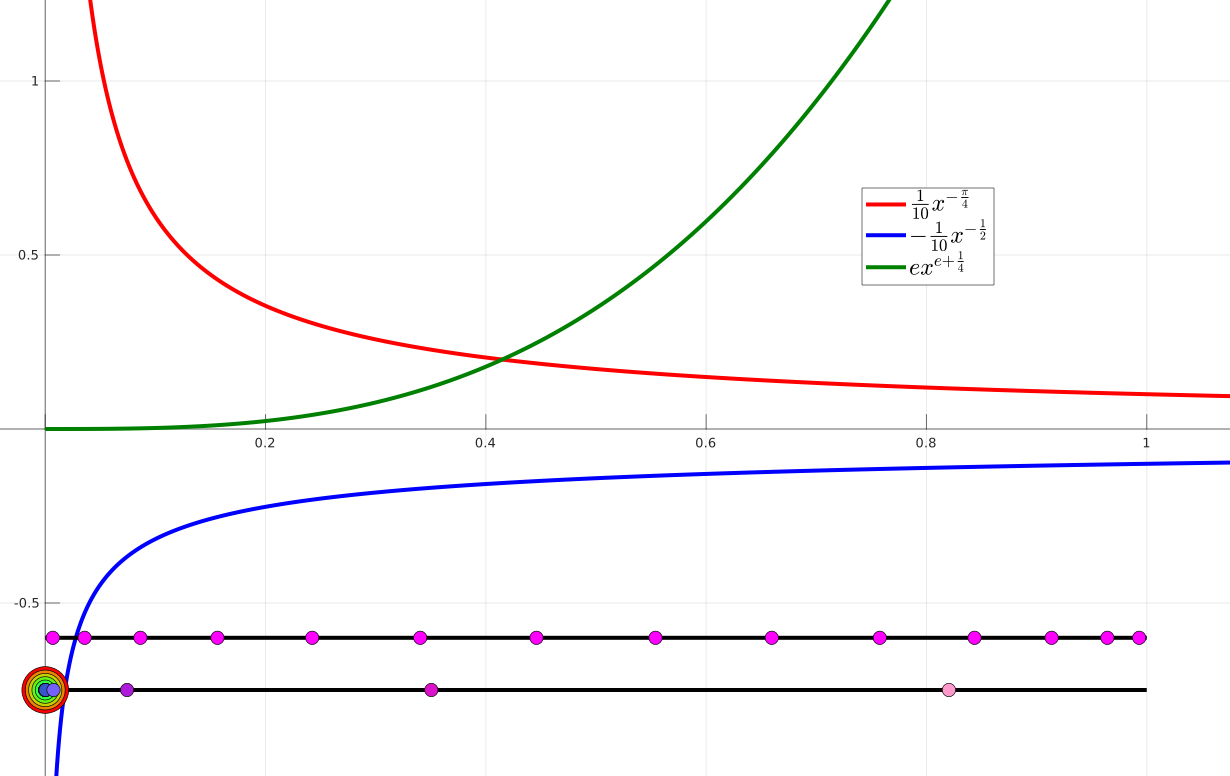
\includegraphics[keepaspectratio, width=\textwidth]{images/GenPolyMonMap.png}
        \caption{This plot shows three singular monomial terms of a Müntz polynomial above. On the bottom of the graph there is the distribution in $[0,1]$ of the $n=14$ nodes of the classical G-L formula (in magenta) and, further below, the new nodes obtained by the monomial quadrature rule (in linear color gradient). Due to the extreme clustering around the infiumum, the latter are progressively scaled down in dimension from $a=0$ to $b=1$. We can clearly see that the linear action of the affine map (\ref{eq1.10}) does not stretch the distribution of the classical G-L nodes which therefore preserve in $[0,1]$ the symmetric property they featured in $[-1,1]$; visually an insufficient number of  nodes $\tilde{x}$ are placed closed to the endpoints of $[0,1]$ where the singularity is, causing a consistent loss in accuracy for the respective quadrature rule. On the other hand, the action of an ad-hoc monomial map (\ref{eq1.13}) to the nodes (whose order $r=28.77$ is given by (\ref{eq1.14}) for the present case) will cluster the vast majority of them around the endpoint singularities of $x^{-\frac{\pi}{4}}$ and $x^{-\frac{1}{2}}$.}
        \label{Fig1.2}
        \end{figure}
\end{center}

\noindent
Considering an instance of such Müntz polynomial

\begin{equation*}
    \Pi(\Lambda)\ni p(x) = ex^{e+\frac{1}{4}} -\frac{1}{10}x^{-\frac{1}{2}} + \frac{1}{10}x^{-\frac{\pi}{4}}\,,\quad\Lambda=\Big\{-\frac{\pi}{4},-\frac{1}{2},e+\frac{1}{3}\Big\}
\end{equation*}

\noindent
a visual representation is reported in Figure \ref{Fig1.2} on the effect that an ad-hoc designed monomial map has on the asymetric redistribution of the G-L quadrature parameters which are listed in Table \ref{table1.2} for reference.

\begin{table}[H]
\centering
\begin{tabular}{|c||c|c|c|c|}
\hline
& \multicolumn{2}{|c|}{\textbf{Classical G-L parameters}}&\multicolumn{2}{|c|}{\textbf{New G-L parameters}}\\
\hline
$j\in\mathbb{N}$ & $x_j\in[0,1]$ & $w_j\in\mathbb{R}^+$ & $x_j\in[0,1]$ & $w_j\in\mathbb{R}^+$ \\
\hline
0   &  0.00685809565159384 &  0.0175597301658759   &  5.58247922741512e-63  & 4.11231619931278e-61  \\
1   &  0.0357825581682132  &  0.0400790435798801   &  2.44695140063495e-42  & 7.88526679349951e-41  \\
2   &  0.0863993424651175  &  0.0607592853439516   &  2.52951532315787e-31  & 5.11781542764354e-30  \\
3   &  0.156353547594157   &  0.0786015835790968   &  6.51929796325047e-24  & 9.42908328714637e-23  \\
4   &  0.242375681820923   &  0.0927691987389689   &  1.95675667095192e-18  & 2.15474891008643e-17  \\
5   &  0.340443815536055   &  0.102599231860648    &  3.44180025480158e-14  & 2.98421017862521e-13  \\
6   &  0.445972525646328   &  0.107631926731579    &  8.13715952769522e-11  & 5.65003223119147e-10  \\
7   &  0.554027474353672   &  0.107631926731579    &  4.18125660540031e-08  & 2.33701617760019e-07  \\
8   &  0.659556184463945   &  0.102599231860648    &  6.30683776156361e-06  & 2.82259817558914e-05  \\
9   &  0.757624318179077   &  0.0927691987389689   &  0.000340288421120315  & 0.00119878736245905  \\
10  &  0.843646452405843   &  0.0786015835790968   &  0.00750950989496675   & 0.0201292451904070  \\
11  &  0.913600657534883   &  0.0607592853439516   &  0.0742930434150393    & 0.142150858859985  \\
12  &  0.964217441831787   &  0.0400790435798801   &  0.350516762468882     & 0.419175839329777  \\
13  &  0.993141904348406   &  0.0175597301658759   &  0.820378484398468     & 0.417316809008697  \\
\hline
\end{tabular}
  \caption{List of all the $n=14$ G-L nodes and weights before (classical) and after the monomial transformation of order $r=28.77$ depicted in Figure \ref{Fig1.2}.}
  \label{table1.2}
\end{table}

 \section[Acknowledgements]{\changefont ACKNOWLEDGEMENTS}\sectionmark{ACKNOWLEDGEMENTS}\label{Sec1.3}

\noindent
This study was supported by the Italian Ministry of University and Research (MIUR) under the PRIN2017 Grant (2017NT5W7Z) \textsl{“Chipless radio frequency identification (RFID) for GREEN TAGging and Sensing - GREEN TAGS"} 

\chapter[Installation]{\Huge \ttfamily INSTALLATION}\chaptermark{INSTALLATION}

In the following chapter we illustrate how to build executable files with QUASIMONT from its source code as well as the dependencies needed at link-time by the resulting application. We begin from the latter issue by outlining the third-party source code necessary for the library prior to the compilation itself. Later a brief description of the organisation and structure of the code is given in order to ease the user interface at compile and link stage. Finally we will address how the library is actually built and illustrate its core features through the execution of proposed test drivers.

\section[Third-party code]{\changefont THIRD-PARTY CODE}\sectionmark{THIRD-PARTY CODE}\label{Sec2.1}

\noindent
The library that we propose is composed by two so-called modules associated with a corresponding \colorbox{poliGrayBlue}{main} function: the primary module, also referred to as the {\itshape focal} module, is the one used by the user to build executables and it implements all the essential methods that are required for the accomplishment of QUASIMONT's purpose, that is the computation of ad-hoc processed nodes and weights of the G-L quadrature formula in order to achieve double precise approximations of a definite integral with the minimum number of nodes possible. The {\itshape secondary} module provides supporting tools for the user to understand deeper the fundamental blocks of the monomial transformation s.a. the plot of the asymptotic estimate $(\ref{eq1.8})$ and the computation of $\beta_{\text{min}}(n)$ and $\beta_{\text{min}}(n)$. Although it is not essential for the correct functioning of the library, it features additional dependencies than the primary module and thus its compilation is kept separate from the rest of the code. In the following we address the building issues concerning the focal module and post-pone to Section \ref{Sec3.4} a brief description of the secondary module.
\newline
\noindent 
QUASIMONT relies on a number of third-party open-source libraries. Many of them usually come shipped with C++ itself e.g. the \color{poliDarkBlue} \textbf{standard} \color{black} and \color{poliDarkBlue} \textbf{vector} \color{black} libraries (required for basic data-structures and functions), the \color{poliDarkBlue} \textbf{algorithm} \color{black} library (needed for sorting methods), the \color{poliDarkBlue} \textbf{math} \color{black} library (used for basic mathematical operations s.a. \colorbox{poliGrayBlue}{fabs}, \colorbox{poliGrayBlue}{pow} and \colorbox{poliGrayBlue}{ceil}) and others. There are however two more libraries, well-known in the scientific computing and open-source communities, that are linked to QUASIMONT (in the following the \color{poliDarkBlue} \textbf{v-number} \color{black} indicates the minimum requirement to run our library):
\begin{itemize}
    \item \color{poliDarkBlue} \textbf{Boost C++ libraries (v-1.71)} \color{black}\cite{boost}: a vast, peer-reviewed, header-only collection whose primary tool in QUASIMONT is the \colorbox{poliGrayBlue}{Multiprecision} library in which non-native higher precision f.p. formats have been implemented as C++ data-types. Of particular interest for our module is the IEEE 754 quadruple f.p. format which is supplied by Boost's library as a {\itshape "GCC's \_\_float128 or Intel's \_Quad data types"}.
    \item \color{poliDarkBlue} \textbf{GSL - GNU Scientific Library (v-2.5)} \color{black}\cite{gsl}: this rather well-known library is needed by QUASIMONT in only one occasion that is for the implementation of the integer degree polynomial solver \colorbox{poliGrayBlue}{gsl\_poly\_complex\_solve}. In the library such method is used to extract the minimum number of quadrature nodes $n_{\text{min}}$ from the $7-$th degree polynomial equation in (\ref{eq1.15}). Alternative solvers and root-finders are available however in our case we were also interest in automatically locating the only real root of such polynomial (corresponding to $n_{\text{min}}$, hence the choice we made.
\end{itemize}

\noindent
Those dependencies need to be installed/compiled correctly on the user's machine; furthermore macros to each static library need to be included in the \colorbox{poliGrayBlue}{PATH} environment variable in order to correctly link the objects files compiled from the source code. Luckily all the above libraries are easily downloaded and compiled in Linux using package managers, such as the \color{poliDarkBlue} \textbf{Advanced Package Tool} \color{black} and the \color{poliDarkBlue} \textbf{Yellowdog Updater, Modified}\color{black}, with a single command on the terminal. Moreover the aforementioned macros should be added automatically to the \colorbox{poliGrayBlue}{PATH} variable.

\vspace{0.5cm}
\begin{tcblisting}{enhanced,
                   arc=5mm,
                   title = \color{black}{\large \ttfamily Installation of third-party libraries},
                   colbacktitle=bashGray,
                   colback=bashBlue,
                   listing only,
                   listing style=BashStyle}
user@machine: home> # For Debian-like distros (Ubuntu, Mint, Knoppix, Kali ...)
user@machine: home> sudo apt-get update -y
user@machine: home> sudo apt-get install libboost-all-dev libgsl-dev
user@machine: home> # For RHEL-like distros (CentOS, Fedora, SUSE, Scientific Linux ...)
user@machine: home> sudo yum update -y
user@machine: home> sudo yum install install boost-devel gsl-devel
\end{tcblisting}
\vspace{0.5cm}

\noindent
Additionally, QUASIMONT requires the proper installation of the appropriate building tools; at the present moment the library has been written for Linux platforms only and therefore we prioritized a minimalist and straightforward build process over cross-platform compliance by adopting the usage of \colorbox{poliGrayBlue}{makefile}s (see Section \ref{Sec2.3}). In it the default compiler specified for compiling and linking QUASIMONT's applications is \color{poliDarkBlue} \textbf{GCC - GNU Compiler Collection} \color{black} \cite{gcc}. The actual program that thus invokes the compilation of the library is \color{poliDarkBlue} \textbf{GNU Make} \color{black} \cite{make} which also requires to be correctly installed configured on the user machine. Also in this case the aforementioned package managers allow fast and simple installation of the tools with minimal input on the terminal.

\vspace{0.5cm}
\begin{tcblisting}{enhanced,
                   arc=5mm,
                   title = \color{black}{\large \ttfamily Installation of building tools},
                   colbacktitle=bashGray,
                   colback=bashBlue,
                   listing only,
                   listing style=BashStyle}
user@machine: home> # For Debian-like distros (Ubuntu, Mint, Knoppix, Kali ...)
user@machine: home> sudo apt-get install build-essential
user@machine: home> gcc --version
user@machine: home> make --version
user@machine: home> # For RHEL-like distros (CentOS, Fedora, SUSE, Scientific Linux ...)
user@machine: home> sudo yum group install "Development Tools"
user@machine: home> gcc --version
user@machine: home> make --version
\end{tcblisting}
\vspace{0.5cm}

\noindent
We remark that QUASIMONT's build has been achieved using versions \colorbox{poliGrayBlue}{9.3.0} and \colorbox{poliGrayBlue}{4.2.1} of GCC and GNU Make respectively. Once all the above packages and tools have been installed, the user should thoroughly check their correct configuration and if indeed links to their static libraries have been added to the \colorbox{poliGrayBlue}{PATH} environment variable. The dependencies are large libraries although QUASIMONT uses a limited amount of the methods they provide; we therefore made sure that only the necessary parts of those were included in the source code, striving to maintain a clean and light final product. For the sake of completeness we hereby list all the methods implemented in those third-party libraries and that are used by QUASIMONT; those can be located in its source code, specifically in the header file \colorbox{poliGrayBlue}{Quasimont.h}, reported in the snippet below. As for any other source file in the library, a comment block precedes the code content, of which the first line specifies the location in the relative tree of the library (see Figure \ref{Fig2.1}).
It can be easily seen that all external source code headers are included in this single header file that takes the name of the library itself; following the definition of the aforementioned custom type it also includes the \textsl{local} headers of the library containing the declarations of all the functions implemented (see Section \ref{Sec2.2}).

\newpage
\vspace{0.5cm}
\tcbinputlisting{enhanced,
                 arc=5mm,
                 title = \color{black}{\large \ttfamily Quasimont.h},
                 colbacktitle=poliOrange,
                 colback=poliGrayBlue,
                 listing only,
                 listing style=CppStyle,
                 listing file=snippets/Quasimont.h}
\vspace{0.5cm}

\noindent
Further down we find definitions of some constants used throughout the library and finally the declaration of leading access point of the primary module of the library, the method \colorbox{poliGrayBlue}{quasimont} in which all other aforementioned methods of QUASIMONT converge and interact. This method is the focal point for all the aforementioned functions and acts as a sort of main-like function that is instead associate to the application itself (see Section \ref{Sec2.3}). The definition of such method is given in the homonym source file \colorbox{poliGrayBlue}{Quasimont.cpp} reported below. With emphasis on the focal module we refer to the latter source file as the {\itshape focal method} (or alternatively the {\itshape access point} from which each application of the library is built). On such file we highlight the comment block at the beginning of the definition of the function itself (lines \colorbox{poliGrayBlue}{18-30}) where the user finds quick useful insights about its usage, I/O and implementation. Such pattern is shared by each method across the main module of the library (see Chapter \ref{Chap4}).

\newpage
\tcbinputlisting{enhanced,
                 arc=5mm,
                 title = \color{black}{\large \ttfamily Quasimont.cpp},
                 colbacktitle=poliOrange,
                 colback=poliGrayBlue,
                 listing only,
                 listing style=CppStyle,
                 listing file=snippets/Quasimont.cpp}
\vspace{0.6cm}

\section[Structure]{\changefont STRUCTURE}\sectionmark{STRUCTURE}\label{Sec2.2}

\noindent
The source-code in the library does not use relative paths for finding the definitions of its methods in the headers; relative paths are instead used at compile and link time by the \colorbox{poliGrayBlue}{makefile} (see Section \ref{Sec2.3}). The user is nonetheless discouraged from moving files and/or changing those paths because they do appear occasionally in the source code for retrieving data from specific non-source files. 
\newline
\noindent 
It is important therefore to understand where these files are stored and how the code is organised. As mentioned in the previous chapters, QUASIMONT is not object-oriented and all its methods interact through the focal method \colorbox{poliGrayBlue}{quasimont} that interfaces the user through the inputs defined in the \colorbox{poliGrayBlue}{main} function. Aprt from it, all the remaining source code that constitutes the primary module of our proposed software is made of only $12$ methods whose definitions are collected in one of the following three source files:
\begin{itemize}
    \item \colorbox{poliGrayBlue}{MonMap.cpp} contains every method associated with the computation of the monomial quadrature rule, ranging from the monomial map itself (i.e. $\beta_{\text{min/max}}$, $r$, etc...) to the quadrature parameters (i.e. $\tilde{x}_j$, $\tilde{w}_j$, $J_{[a,b]}$, etc...). To provide an easier reference for code debugging and amendment, a naming scheme of these methods is adopted; every function in this file is in fact named \color{poliDarkBlue} \textbf{compute}$\boldsymbol{<}$\textbf{NameOfFunction$\boldsymbol{>}$} \color{black} as it can be evinced from the corresponding header file containing such functions' declarations
    \tcbinputlisting{enhanced,
                 arc=5mm,
                 grow to left by=8mm, 
                 title = \color{black}{\large \ttfamily MonMap.h},
                 colbacktitle=poliOrange,
                 colback=poliGrayBlue,
                 listing only,
                 listing style=CppStyle,
                 listing file=snippets/MonMap.h}
                 
    \item \colorbox{poliGrayBlue}{DatIo.cpp} is the source file defining each method that does not perform raw computations but instead manages the data flow e.g. in I/O operations. Every function follows the naming scheme \color{poliDarkBlue} $\boldsymbol{<}$\textbf{NameOfFunction$\boldsymbol{>}$}\textbf{Data} \color{black} emphasizing its characteristics of data manipulation method. The methods are declared in the corresponding header file
    \vspace{0.5cm}
    \tcbinputlisting{enhanced,
                 arc=5mm,
                 grow to left by=8mm,
                 title = \color{black}{\large \ttfamily DatIo.h},
                 colbacktitle=poliOrange,
                 colback=poliGrayBlue,
                 listing only,
                 listing style=CppStyle,
                 listing file=snippets/DatIo.h}
    \vspace{0.5cm}
    \item \colorbox{poliGrayBlue}{VecOps.cpp} finally defines every function that does not either perform direct computations for the quadrature rule nor it performs I/O operations on data; instead the methods instantiated from the source file are used to automatise specific operations on vectors that are required multiple times across the library specifically casting vectors' values in \textsl{higher-than-double} floating-point format (implemented in method in \colorbox{poliGrayBlue}{castVector}) and the \colorbox{poliGrayBlue}{doubleDotProduct} which implements a precise inner product operation between two non-scalar vectors with high precision avoiding numerical cancellations of smaller-than-epsilon values. Given the generic nature of their task, no naming scheme is assigned to these methods whose declarations are found in the header file \colorbox{poliGrayBlue}{Utils.h} below. In the latter we also find declarations of the $3$ methods of the secondary module that are all defined, alongside its \colorbox{poliGrayBlue}{main}, in the \colorbox{poliGrayBlue}{ErrTools.cpp} source file (see Section \ref{Sec3.4}).
    
    \newpage
    \vspace{0.5cm}
    \tcbinputlisting{enhanced,
                 arc=5mm,
                 grow to left by=8mm,
                 grow to right by=2mm,
                 title = \color{black}{\large \ttfamily Utils.h},
                 colbacktitle=poliOrange,
                 colback=poliGrayBlue,
                 listing only,
                 listing style=CppStyle,
                 listing file=snippets/Utils.h}
\end{itemize}

\noindent
Now that we have a clearer idea of the actual content of QUASIMONT source code let us discuss, with visual reference depicted in Figure \ref{Fig2.1}, the organisation of each file in the library's directory. Source files of the primary module, i.e. \colorbox{poliGrayBlue}{MonMap.cpp} and \colorbox{poliGrayBlue}{DatIo.cpp} are located in the subdirectory \colorbox{poliGrayBlue}{\textbf{QUASIMONT/src}} alongside \colorbox{poliGrayBlue}{Quasimont.cpp} itself. On the other hand \colorbox{poliGrayBlue}{VecOps.cpp} is placed in the \colorbox{poliGrayBlue}{\textbf{QUASIMONT/utilities}} subdirectory where we can also find the secondary module source code \colorbox{poliGrayBlue}{ErrTools.cpp}. Despite such separation, all the header files outlined above (one per source file of the focal module) are located in the \colorbox{poliGrayBlue}{\textbf{QUASIMONT/include}} subdirectory, including \colorbox{poliGrayBlue}{Quasimont.h}. Now we discuss the aforementioned relative paths; we mentioned that they are essentials for the correct loading of raw data from \color{poliDarkBlue} \textbf{tabulated data-files} \color{black} into the source code.

\newpage
\begin{center}
        \begin{figure}[H]
        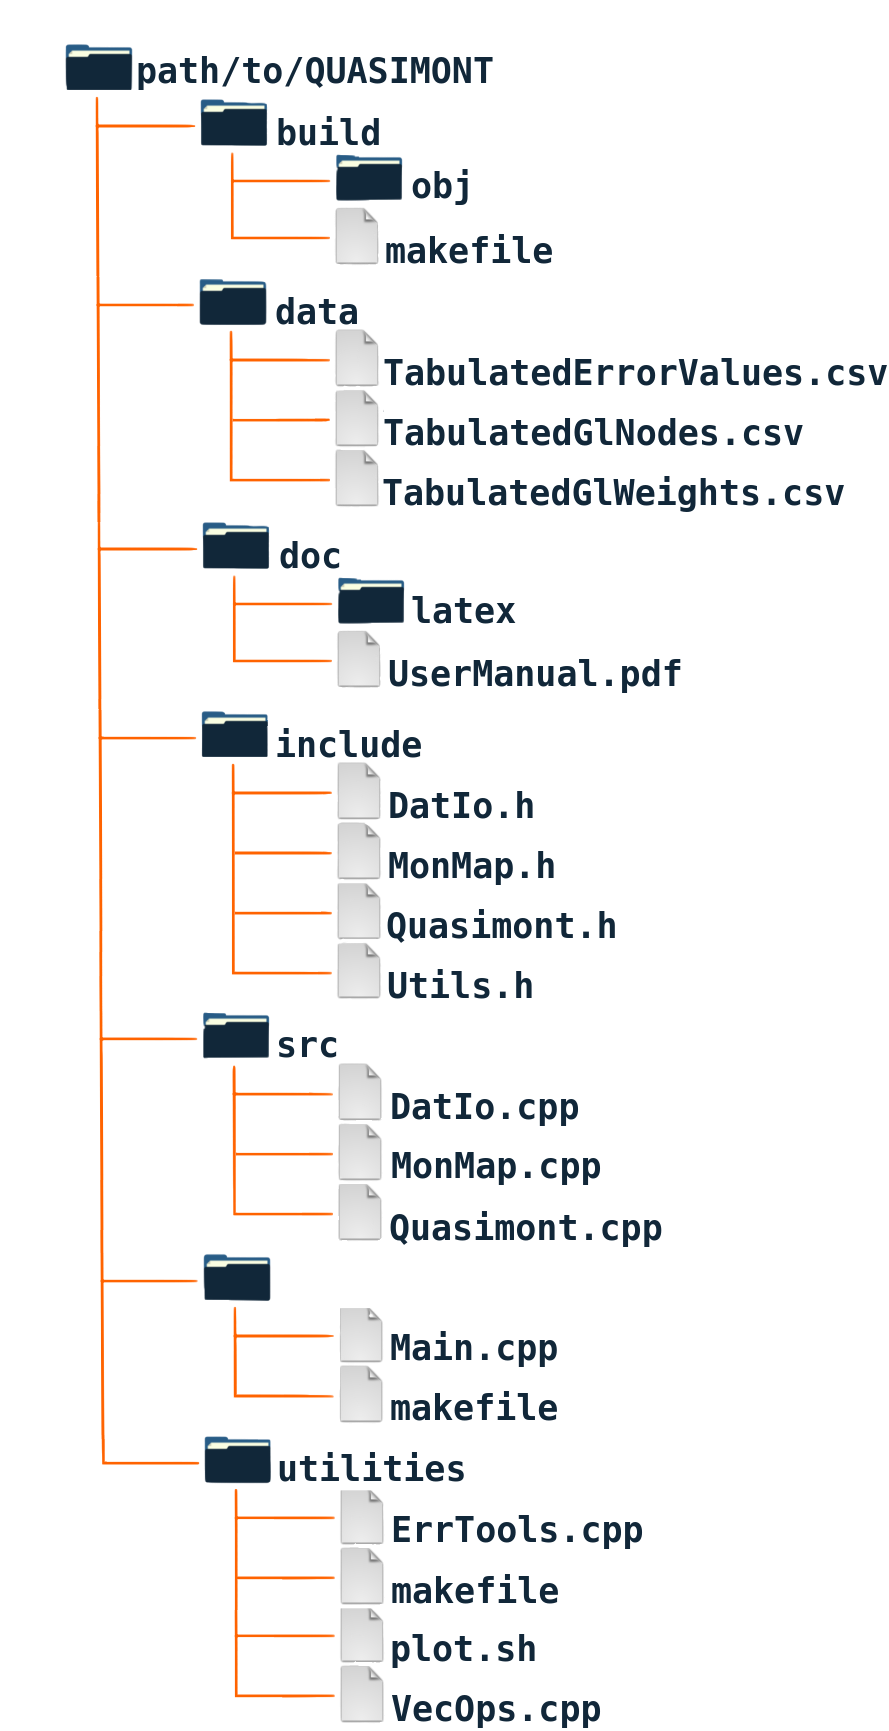
\includegraphics[keepaspectratio, height=\textheight]{images/DirectoryStructure.png}
        \caption{A directory tree representing the structure and organisation of QUASIMONT}
        \label{Fig2.1}
        \end{figure}
\end{center}

\newpage
\noindent 
 Those files are:
\begin{itemize}
    \item \colorbox{poliGrayBlue}{TabulatedErrorValues.csv} collecting the values of $\beta_{\text{min}}(n)$ and $\beta_{\text{max}}(n)$ for each even value of $n\in[10,100]$;
    \item \colorbox{poliGrayBlue}{TabulatedGlNodes.csv} storing the G-L quadrature nodes in $[-1,1]$ for each even value of $n\in[10,100]$;
    \item \colorbox{poliGrayBlue}{TabulatedGlWeights.csv} storing the strictly positives, symmetric (w.r.t. to $0$) weights of the G-L quadrature formula for each even value of $n\in[10,100]$.
\end{itemize}
Those files are located in \colorbox{poliGrayBlue}{\textbf{QUASIMONT/data}} and shall never be changed. In the \colorbox{poliGrayBlue}{\textbf{QUASIMONT/build}} the \colorbox{poliGrayBlue}{makefile} used for building the library and its applications is located whereas \colorbox{poliGrayBlue}{\textbf{QUASIMONT/build/obj}} subdirectory contains the object files created at compile-time. Finally, test drivers (see Section \ref{Sec2.4}) used for checking the proper installation and execution of the application are located in \colorbox{poliGrayBlue}{\textbf{QUASIMONT/test}}.

\section[Build process]{\changefont BUILD PROCESS}\sectionmark{BUILD PROCESS}\label{Sec2.3}

\noindent
The principle by which QUASIMONT is used is that of creating executables, henceforth referred to as \color{poliDarkBlue} \textbf{applications}\color{black}, through the compilation and linking of the library's source code and a \colorbox{poliGrayBlue}{Main.cpp} file containing the user's input thus called \color{poliDarkBlue} \textbf{input source file} \color{black} (see Section \ref{Sec3.1}). We define a one-to-one correspondence between any specific \colorbox{poliGrayBlue}{main} of the primary module and its associated application. 

    \tcbinputlisting{enhanced,
                 arc=5mm,
                 title = \color{black}{\large \ttfamily Application's own (top-level) makefile},
                 colbacktitle=poliOrange,
                 colback=poliGrayBlue,
                 listing only,
                 listing style=MakeStyle,
                 listing file=snippets/makefile}

\noindent
The build process is based on the \textsl{recursive make} approach, i.e. the input source file is built through a top-level \colorbox{poliGrayBlue}{makefile} that recursively invokes the \colorbox{poliGrayBlue}{makefile} responsible for building the source code of the library, its utilities and third-party dependencies. The library source code shall be compiled just once and be available thereafter for linking each new application unless the rule \colorbox{poliGrayBlue}{allclean} is invoked (which deletes the library's object files). This practice is useful for users of the library that only require to execute standalone applications and can thus reuse the compiled objects of the source code multiple times with no changes. On the other hand, if integration of QUASIMONT in larger, more complex code is required (e.g. in FEM/BEM libraries), linking to the static library is necessary. It is later explained in Section \ref{Sec2.4} that QUASIMONT is shipped with a reference application in \colorbox{poliGrayBlue}{\textbf{QUASIMONT/test}}  which, among other things, exemplifies the build sequence of the library. 

\vspace{0.5cm}
\begin{tcblisting}{enhanced,
                   arc=5mm,
                   title = \color{black}{\large \ttfamily Compilation and Linking of the library},
                   colbacktitle=bashGray,
                   colback=bashBlue,
                   listing only,
                   listing style=BashStyle}
# First clean the object files from any previous compilation ...
user@machine: home/QUASIMONT/UserApplication_dir> make allclean
cd ../build && make clean
make[1]: Entering directory '/home/QUASIMONT/build'
rm -f obj/*.o
make[1]: Leaving directory '/home/QUASIMONT/build'
# ... then builds the library object files
user@machine: g++ -c Main.cpp -o ../build/obj/Main.o -ansi -std=c++17 -I ../include
cd ../build && make
make[1]: Entering directory '/home/QUASIMONT/build'
g++ -c ../src/Quasimont.cpp -o obj/Quasimont.o -g -ansi -std=c++17 -I ../include 
g++ -c ../src/DatIo.cpp -o obj/DatIo.o -g -ansi -std=c++17 -I ../include 
g++ -c ../src/MonMap.cpp -o obj/MonMap.o -g -ansi -std=c++17 -I ../include 
make[1]: Leaving directory '/home/QUASIMONT/build'
cd ../utilities && make ../build/obj/VecOps.o
make[1]: Entering directory '/home/QUASIMONT/utilities'
g++ -c VecOps.cpp -o ../build/obj/VecOps.o -g -ansi -std=c++17 -I ../include 
make[1]: Leaving directory '/home/QUASIMONT/utilities'
# ... and finally links all together to create the executable ...
g++ ../build/obj/*.o -o Test -lm -lquadmath -lgsl -lgslcblas
# ... which is then ran!
./Test

    |----------------------------------|
    |          ** QUASIMONT **         |
    |  ** MONOMIAL QUADRATURE RULE **  |
    |----------------------------------|


 Input polynomial...
\end{tcblisting}
\vspace{0.5cm}

\noindent
The output of the compilation of the source files are object files that will be stored in the \colorbox{poliGrayBlue}{\textbf{QUASIMONT/build/obj}} subdirectory as explained previously. The linking of those objects is invoked only by the top-level makefile associated to the specific application. For each application built by the user it is considered a good practice to invoke the \colorbox{poliGrayBlue}{clean} rule prior to the build process itself, as shown above. We emphasize that, with the exception of those cases when QUASIMONT is used as a tool in a larger library, each application should be associated to its own subdirectory located within QUASIMONT itself. In this subdirectory a user input source file containing the \colorbox{poliGrayBlue}{main}, named \colorbox{poliGrayBlue}{Main.cpp} by default, should be located. User can name it whatever it wants as long as it is consistent with the one reported in the top-level \colorbox{poliGrayBlue}{makefile} of the application, which should also be located in the subdirectory. Nonetheless we suggest to retain the naming convention reported in the \colorbox{poliGrayBlue}{makefile} above, that is the application (\colorbox{poliGrayBlue}{Test} in our example above) should be name according to the directory in which is located (i.e. \colorbox{poliGrayBlue}{\textbf{test}}) whereas the input source file should be always named \colorbox{poliGrayBlue}{Main.cpp} to provide easier reference for debugging.

\newpage
\section[Installation and test driver]{\changefont INSTALLATION AND TEST DRIVER}\sectionmark{INSTALLATION AND TEST DRIVER}\label{Sec2.4}

\noindent
Installation of the library can be done by building the \colorbox{poliGrayBlue}{Main.cpp} input source file in the \colorbox{poliGrayBlue}{\textbf{QUASIMONT/test}} subdirectory, which contains the test driver benchmarking QUASIMONT's performance. The \colorbox{poliGrayBlue}{Test} application built from it runs the library's processing methods onto three generalised and classical polynomial integrands that introduce the user to the library interaction, execution and output whilst assuring that the core functionalities have been compiled correctly (no conflict at linking stage occurs). The three polynomial functions are the following

\begin{equation*}
    \begin{split}
        p_1(x) & = 5x^{-\frac{\pi}{4}}-x^{-\frac{1}{2}}+1+10x^{2}+ex^{e+\frac{1}{4}} \\
        p_2(x) & = x^{-\frac{e}{3}} \\
        p_3(x) & = x^{17} + x^{35}
    \end{split}
\end{equation*}

\noindent
and, with the exception of $p_3(x)$, all have a singularity in $[0,1]$, which is also the integration interval set by default in QUASIMONT. Once both the library's and user input's source files have been compiled and linked into the corresponding executable, the resulting application integrates each polynomial using the monomial quadrature rule; a list of important information regarding both the I/O and the monomial transformation itself is displayed on the terminal whereas the main results, which we emphasize to be the new processed G-L quadrature nodes and weights, are exported in the associated subdirectory (see Section \ref{Sec3.2}). The user should check its content and verify that the data contained in it matches what is reported in the following tables \ref{table2.1}, \ref{table2.2}, \ref{table2.3} for the specific polynomial functions. Once satisfied the user can then return to the CLI where the program is waiting for her/him to go ahead to the next benchmark.

\vspace{0.5cm}
\begin{tcblisting}{enhanced,
                   arc=5mm,
                   title = \color{black}{\large \ttfamily Building and executing the test driver: p\_1(x)},
                   colbacktitle=bashGray,
                   colback=bashBlue,
                   listing only,
                   listing style=BashStyle}
user@machine: home/QUASIMONT/test> make clean
rm -f ../build/obj/Main.o Test
rm -r output
user@machine: home/QUASIMONT/test> make
g++ -c Main.cpp -o ../build/obj/Main.o -g  -I ../include
cd ../build && make
make[1]: Entering directory '/home/QUASIMONT/build'
g++ -c ../src/Quasimont.cpp -o obj/Quasimont.o -g -I ../include 
g++ -c ../src/DatIo.cpp -o obj/DatIo.o -g -I ../include 
g++ -c ../src/MonMap.cpp -o obj/MonMap.o -g -I ../include 
make[1]: Leaving directory '/home/QUASIMONT/build'
cd ../utilities && make ../build/obj/Utils.o
make[1]: Entering directory '/home/QUASIMONT/utilities'
g++ -c Utils.cpp -o ../build/obj/Utils.o -g -I ../include
make[1]: Leaving directory '/home/QUASIMONT/utilities'
g++ ../build/obj/*.o -o Test -lm -lgsl -lgslcblas -lgmp -lquadmath
./Test

    |----------------------------------|
    |  ** MONOMIAL QUADRATURE RULE **  |
    |----------------------------------|


 Input polynomial p(x) = +2.71828*x^(2.96828)+5*x^(-0.785398)-1*x^(-0.5)+x^(0) +10*x^(2)

 ** Accepted sequence of exponents ** 
    {2.96828, -0.785398, -0.5, 0, 2}
 ** Lambda_min = -0.785398, Lambda_max = 2.96828 **
 --------------------------------------------------
 ** Beta_min = 4.37782518, Beta_max = 127.894326 **
 ** Transformation order = 28.770346 **
 --------------------------------------------------
 ** Using double format for nodes and weights
 ** I_n(p(x)) = 26.3172973764883195713082386646419764 **
 ** E_n(p(x)) = 1.34995384517502488806263407884576529e-16 **


PROGRAM TERMINATED! Results are available in the 'output' subdirectory.
Press any Key to exit
\end{tcblisting}
\vspace{0.5cm}

\noindent
The correct execution of all three benchmarks will then close the application. The user should check that each benchmark is executed without problems and the results are correctly generated (see Section \ref{Sec3.2}). As for the the quality of the results obtained for those tests, an in-depth analysis, coupled with the fast execution of the program, shows the advantages provided by QUASIMONT over classical G-L and other generalised quadrature rules. The first polynomial $p_1(x)$ is a model proposed at equation (73) in \cite{Lombardi09}, \textsl{Section 5.1. Example 1} and it represents the quintessential integrand function, often encountered in the numerical methods for differential and integral equations, on which QUASIMONT is deemed necessary. The generalised polynomial feature a strong singulairty in the infimum of the interval and all but one of its monomial terms have non-integer degree. The numerical approximation of the integral is achieved with $n=32$ nodes using a monomial transformation of high order of the classical G-L nodes and weights in $[0,1]$.

\begin{table}[H]
\centering
\begin{tabular}{|c||c|c|}
\hline
\multicolumn{3}{|c|}{\textbf{Transformed G-L nodes and weights (double f.p. format)}} \\
\hline
$j\in\mathbb{N}$ & $x_j\in[0,1]$ & $w_j\in\mathbb{R}^+$ \\
\hline
0   &  4.0256721894941735e-83  &  2.9709584266857193e-81  \\
1   &  2.2116841854653406e-62  &  7.1971053989801097e-61  \\
2   &  3.4370358897566318e-51  &  7.1255611223692978e-50  \\
3   &  1.6010758830624544e-43  &  2.4253789034229506e-42  \\
4   &  1.0479208102676717e-37  &  1.2456363438765983e-36  \\
5   &  4.8718071131884711e-33  &  4.7453741025535338e-32  \\
6   &  3.7119919463646725e-29  &  3.0494845207591382e-28  \\
7   &  7.5510919371932376e-26  &  5.3393428605147779e-25  \\
8   &  5.58947068987428e-23    &  3.4526789629984772e-22  \\
9   &  1.8549840400142102e-20  &  1.0121884313459638e-19  \\
10  &  3.1981531227726135e-18  &  1.5545919457374846e-17  \\
11  &  3.1905126409913618e-16  &  1.3904418738462426e-15  \\
12  &  1.9974633805093215e-14  &  7.8421013950383668e-14  \\
13  &  8.3548669580378659e-13  &  2.9653252968844048e-12  \\
14  &  2.4525558094710645e-11  &  7.8879379262599627e-11  \\
15  &  5.2553535644885825e-10  &  1.5337625816699302e-09  \\
16  &  8.4865615532959245e-09  &  2.2485149221054993e-08  \\
17  &  1.0601166175497224e-07  &  2.5487504629916981e-07  \\
18  &  1.0467771915132323e-06  &  2.2805293469267595e-06  \\
19  &  8.3187859060800558e-06  &  1.6383778757563812e-05  \\
20  &  5.4017656350748472e-05  &  9.583886949817516e-05   \\
21  &  0.00029027719974030597  &  0.00046172220499588948  \\
22  &  0.0013048618829373392   &  0.0018488842315729846   \\
23  &  0.0049515587664587246   &  0.0061972140073356637   \\
24  &  0.01598386920155067     &  0.017474549464975012    \\
25  &  0.044176504650425052    &  0.041563995305652503    \\
26  &  0.10510275956828145     &  0.083385319613667491    \\
27  &  0.21621415218381346     &  0.14051580648196024     \\
28  &  0.38598199665949656     &  0.19670495174814193     \\
29  &  0.59964365548997856     &  0.22295968412650397     \\
30  &  0.81242716007987004     &  0.1915755472071223      \\
31  &  0.96137880664253184     &  0.097197543454586643    \\
\hline
\end{tabular}
  \caption{New G-L nodes and weights obtained by a monomial transformation of order $r=28.77$ integrating $p_1(x)$ in $[0,1]$.}
  \label{table2.1}
\end{table}

\noindent
From the table above it is easy to get a sense on what was displayed in the previous Figure \ref{Fig1.2}; the classical nodes G-L nodes of the associated quadrature rule with $n=32$ are in fact distributed symmetrically in $[0,1]$ with an equal abundance of those at both bounds of the integration interval. Conversely here, the monomial transformation order shifts those nodes consistently towards the lower bound $a=0$, squashing the vast majority of them ($26$ out of the total $32$) inside the sub-interval $[0,0.1]$ where the singularity is captured. Onto the second polynomial, it is proposed with the purpose of introducing the user to a core functionality of QUASIMONT that requires further input on the CLI. We see in fact that $p_2(x)$ is a monomial of non-integer degree and, as stated in Section \ref{Sec1.1}, their numerical integration requires careful manipulation. During the modelling process of larger applications, especially when dealing with finite elements constructed over triangulations of domains with singular spatial geometries, there may in fact arise the need of integrating low order, singular and hyper-singular polynomial basis functions. One straightforward workaround, which is in actuality often encountered in many of those problems, is the addition of a higher-order monomial function. In QUASIMONT we allow for the insertion of such term by identifying its degree as $\lambda_{\text{max}}$; the additional monomial will have a unitary coefficient by default and can indeed be the constant $x^0=+1$ itself. The integration is enabled using a caveat prompted on the terminal and it consists in choosing one path between two mutually exclusive options that the user must exercise in order to continue with the application. One of those is the choice of specifying the maximum number $n$ of nodes it wants for the quadrature rule, in which case the library will automatically compute $\lambda_{\text{max}}$  and thus integrate $\tilde{p_2}(x) = x^{-\frac{e}{3}} + x^{\lambda_\text{max}}$. The second path allows instead to specify $\lambda_{\text{max}}$ directly and let QUASIMONT carry out the integration.

\begin{tcblisting}{enhanced,
                   arc=5mm,
                   title = \color{black}{\large \ttfamily Building and executing the test driver: p\_2(x)},
                   colbacktitle=bashGray,
                   colback=bashBlue,
                   listing only,
                   listing style=BashStyle}

** E_n(p(x)) = 1.34995384517502488806263407884576529e-16 **


PROGRAM TERMINATED! Results are available in the 'output' subdirectory.
Press any Key to exit 


    |----------------------------------|
    |  ** MONOMIAL QUADRATURE RULE **  |
    |----------------------------------|


 Input polynomial p(x) = +x^(-0.906093942819681745120095823784220804) 

   ** WARNING ** Your input is a monomial of non-integer degree
                 You need at least a binomial to achieve double-precision quadrature
                 How do you want to proceed?
   [enter 'nodes' to specify the number of nodes or 'lambda' for the exponent]

                 Input: 

\end{tcblisting}

It is easy to see that the second case essentially reduces to a \textsl{"standard"} polynomial input, as far as the library is concerned. Therefore we suggest the user to go ahead with the former option and specify the maximum $n$ for which its singular monomial can be integrated. The user should therefore type \colorbox{poliGrayBlue}{nodes} on the CLI and press Enter; we are now prompted to select any value of $n\in[10,100]$; user should type 12 and press Enter again. On the contrary typing \colorbox{poliGrayBlue}{lambda} will cause the application to resort to its original workflow with the intermediate step of requiring the input of the value of $\lambda_{\text{max}}$ with the \colorbox{poliGrayBlue}{.} character separating the integer from the decimal entries.

\begin{tcblisting}{enhanced,
                   arc=5mm,
                   title = \color{black}{\large \ttfamily Building and executing the test driver: p\_2(x)},
                   colbacktitle=bashGray,
                   colback=bashBlue,
                   listing only,
                   listing style=BashStyle}
                   
How do you want to proceed?
   [enter 'nodes' to specify the number of nodes or 'lambda' for the exponent]

                 Input: nodes


Please specify the desired number of quadrature nodes (number must be even): 12
 --------------------------------------------------
 ** Beta_min = 8.54130275, Beta_max = 23.2002133 **
 ** Accepted sequence of exponents ** 
    {-0.906093942819681745120095823784220804, -0.761820098074495688500462620140751824}
 ** Lambda_min = -0.906093942819681745120095823784220804, Lambda_max = -0.761820098074495688500462620140751824 **
 --------------------------------------------------
 ** Beta_min = 8.54130275, Beta_max = 23.2002133 **
 ** Transformation order = 101.604763 **
 --------------------------------------------------
 ** Using float50 format for nodes and weights
 ** I_n(p(x)) = 14.8474473958169998935662658402046966 **
 ** E_n(p(x)) = 3.02455261304583008416598346191664263e-16 **


PROGRAM TERMINATED! Results are available in the 'output' subdirectory.
Press any Key to exit
\end{tcblisting}

We make the remark that any miss-typed or empty input, will cause QUASIMONT to throw an error message and exit the program. As we can see QUASIMONT computes automatically a value of $\lambda_{\text{max}} = -0.761820098074$ and the resulting quadrature retains the machine-epsilon double precision. Here The library is stressed more as its transformation order gains an order of magnitude; the effects are registered on the mapped nodes and weights listed in the following table.

\begin{table}[H]
\centering
\begin{tabular}{|c||c|c|}
\hline
\multicolumn{3}{|c|}{\textbf{Transformed G-L nodes and weights (double f.p. format)}} \\
\hline
$j\in\mathbb{N}$ & $x_j\in[0,1]$ & $w_j\in\mathbb{R}^+$ \\
\hline
0   &  1.6049071040670031e-207  &  4.1718913867161883e-205  \\
1   &  8.9928778579205101e-135  &  1.0190834572864527e-132  \\
2   &  3.8114927390083667e-96   &  2.6942018712200615e-94   \\
3   &  2.2836535914412963e-70   &  1.1423068956574762e-68   \\
4   &  1.5051778942712652e-51   &  5.6486159643104545e-50   \\
5   &  3.2351037993447086e-37   &  9.3619397179684863e-36   \\
6   &  4.1726571491647704e-26   &  9.3872826135408085e-25   \\
7   &  1.7198033365919789e-17   &  2.9828626539946124e-16   \\
8   &  6.3435088215964896e-11   &  8.2496166241381113e-10   \\
9   &  4.0434975152747609e-06   &  3.7158177341626430e-05   \\
10  &  0.0067940636342241       &  0.0387692527955493       \\
11  &  0.3901949656940479       &  0.9438508439664283       \\
\hline
\end{tabular}
  \caption{New G-L nodes and weights obtained by a monomial transformation of order $r=101.6$ integrating $p_2(x)$ in $[0,1]$.}
  \label{table2.2}
\end{table}

\noindent
The reason for such an extreme value of the map is that we specified the maximum number of quadrature nodes to be used is $n=12$; such value force the algorithm to compress the region of finite-arithmetic exactness to a very narrow sub-interval of $\lambda\in(-1,+\infty)$ and hence the extreme pinching of the G-L nodes on the lower bound $a=0$. Finally, with the last benchmark a classical polynomial of high integer-degree is integrated following the processing of the G-L nodes and weights. As $p_3(x)$ is a binomial, the standard path of QUASIMONT is ran. According to the properties described in Section \ref{SubSec1.2.2}, it would only require $n=\frac{d+1}{2}=18$ nodes for the classical G-L quadrature to achieve double precise integration.

\vspace{0.5cm}
\begin{tcblisting}{enhanced,
                   arc=5mm,
                   title = \color{black}{\large \ttfamily Building and executing the test driver: p\_3(x)},
                   colbacktitle=bashGray,
                   colback=bashBlue,
                   listing only,
                   listing style=BashStyle}
                   
    |----------------------------------|
    |  ** MONOMIAL QUADRATURE RULE **  |
    |----------------------------------|


 Input polynomial p(x) = +x^(17) +x^(35) 

 ** Accepted sequence of exponents ** 
    {17, 35}
 ** Lambda_min = 17, Lambda_max = 35 **
 --------------------------------------------------
 ** Beta_min = 8.54130275, Beta_max = 23.2002133 **
 ** Transformation order = 0.601150 **
 --------------------------------------------------
 ** Using float128 format for nodes and weights
 ** I_n(p(x)) = 0.083333333333333325939326815805736207 **
 ** E_n(p(x)) = 8.87280782103311654675619815821351188e-17 **


PROGRAM TERMINATED! Results are available in the 'output' subdirectory.
Press any Key to exit
# User shall press 'Enter' twice in this case
user@machine: home/QUASIMONT/test>
\end{tcblisting}
\vspace{0.5cm}

\noindent
Yet we immediately notice that QUASIMONT outperforms such result using even less samples in $[0,1]$, i.e. $n=12$; also the transformation order needed by the monomial map is significantly lower than the previous two cases. The integer degrees of the integrand function thus makes the polynomial suitable to very little rearrangement of the classical nodes distribution and weights positive values in order to achieve a numerical approximation that is accurate within the machine-epsilon. This can be assessed by the table below by how close those processed values are, w.r.t. the classical G-L nodes in $[0,1]$, when compared to those of the previous generalised cases of $p_1(x)$ and $p_2(x)$.

\begin{table}[H]
\centering
\begin{tabular}{|c||c|c|}
\hline
\multicolumn{3}{|c|}{\textbf{Transformed G-L nodes and weights (double f.p. format)}} \\
\hline
$j\in\mathbb{N}$ & $x_j\in[0,1]$ & $w_j\in\mathbb{R}^+$ \\
\hline
0   &  0.0597707229696358   &  0.0919264663553836  \\
1   &  0.1610307309568925   &  0.1079664407846363  \\
2   &  0.2725515941208583   &  0.1139863183561349  \\
3   &  0.3872246099856674   &  0.1145999654489373  \\
4   &  0.5003873977306973   &  0.1111039615531504  \\
5   &  0.6082809536783961   &  0.1041479683059256  \\
6   &  0.7076854327640707   &  0.0941968566214454  \\
7   &  0.7958143666363263   &  0.0816648573999376  \\
8   &  0.8702918448156044   &  0.0669634924046180  \\
9   &  0.9291601555462656   &  0.0505192348221430  \\
10  &  0.9708981507831240   &  0.0327793590987762  \\
11  &  0.9944473508291223   &  0.0142322139984140  \\
\hline
\end{tabular}
  \caption{New G-L nodes and weights obtained by a monomial transformation of order $r=0.6011$ integrating $p_3(x)$ in $[0,1]$.}
  \label{table2.3}
\end{table}

\noindent
With these results we would like to direct the user attention on the possibility of using QUASIMONT even for standard/classical polynomials of integer degree as its processed nodes and weights will most likely lead to a fewer samples in the quadrature rule and thus more efficient code in the numerical analysis of complicated physical models. At the best of our knowledge, and based on the tests reported here and in \cite{Lombardi09, Lombardi21}, the monomial transformation can be adapted to the widest range of generalised polynomial of non-integer degree as long as the constraint of $\lambda_{\text{min}}>-1$ holds for the integrand. By excluding those cases of rational functions we argue that the usage of QUASIMONT produces accurate results faster (using the minimum possible number of samples) and more efficiently (outputting the most optimised f.p. formats for the G-L quadrature parameters) than any other algorithm that currently deals with both classical and singular polynomial integrands of either integer and/or non-integer degree. As a final important observation, we note that QUASIMONT uses tabulated values of the original G-L nodes and weights in $[-1,1]$ with $50$ decimal digits of precision; the automatisation of those is outside the scope of the library and already explored in details and implemented in other works \cite{Gautschi94,Hale13}.

\chapter[User interface]{\Huge \ttfamily USER INTERFACE}\chaptermark{USER INTERFACE}

The execution of the test drivers should have introduced the user on the fundamentals and interaction with the library. It is now time to expose its I/O interface and enabling the user to the creation of a quick application. In the following chapter we shall provide a step-by-step procedure to setup, build and execute a custom-made application from scratch. In the first section we discuss the input source file, amendable by the user to create her/his first application with the library. In the second section we address how the results are exported. Finally we briefly address how these results can be used by other applications and loaded in external code automatically by integrating QUASIMONT in a larger library and conclude with a brief touch on the secondary module of our library.

\section[The input source file]{\changefont THE INPUT SOURCE FILE}\sectionmark{THE INPUT SOURCE FILE}\label{Sec3.1}

Let us start with an example; we would like to integrate the following singular polynomial 
\begin{equation*}
    p(x) = x^{\frac{\pi}{2}} + x^{\frac{\pi}{3}} + x + x^{\frac{\pi}{6}} + 1\,,\quad x\in[0,1]
\end{equation*}
which is reported in \textsl{Section 5.6. Example 6} in \cite{Lombardi09}. We start by creating a new source file collecting our inputs. By recalling \colorbox{poliGrayBlue}{Main.cpp} in the \colorbox{poliGrayBlue}{\textbf{QUASIMONT/test}} subdirectory we can create a copy of the whole subdirectory and rename it accordingly, e.g. \colorbox{poliGrayBlue}{\textbf{QUASIMONT/MyApp}}

\vspace{0.5cm}
\begin{tcblisting}{enhanced,
                   arc=5mm,
                   title = \color{black}{\large \ttfamily Creation of application's directory},
                   colbacktitle=bashGray,
                   colback=bashBlue,
                   listing only,
                   listing style=BashStyle}
user@machine: home/QUASIMONT> cp -r test MyApp
user@machine: home/QUASIMONT> cd MyApp/
user@machine: home/QUASIMONT> rm -r output/ Test
\end{tcblisting}
\vspace{0.5cm}

\noindent
Now that a new application directory exists it is necessary to change our inputs in both the input source file and the associated top-level \colorbox{poliGrayBlue}{makefile}. We start from the latter for which the amendments amount to

\begin{itemize}
    \item at lines \colorbox{poliGrayBlue}{33}, \colorbox{poliGrayBlue}{34} and \colorbox{poliGrayBlue}{46} (see the code snippet in Section \ref{Sec2.3}) change the string \colorbox{poliGrayBlue}{Test} to \colorbox{poliGrayBlue}{MyApp} to effectively rename the application built by the compiler;
    \item alternatively at line \colorbox{poliGrayBlue}{31} define a macro variable \colorbox{poliGrayBlue}{EXE\_NAME = MyApp} and invoke it as \colorbox{poliGrayBlue}{\$(EXE\_NAME)} at the corresponding lines above.
\end{itemize}

\noindent
With regards to the input source file we must \colorbox{poliGrayBlue}{Main.cpp} in a text editor or IDE and observe the content of the test driver; going ahead and delete the comment block at lines \colorbox{poliGrayBlue}{1-14} and all the code in the \colorbox{poliGrayBlue}{main} will prepare it for our next inputs. We remind that QUASIMONT is designed to perform its operations on generalised polynomials with strong endpoint singularities in $[0,1]$ therefore, by using such bounds as the default integration interval, the library only requires the user to uniquely specify its input i.e.

\begin{itemize}
    \item the \colorbox{poliGrayBlue}{coefficients\_sequence} stored in a \colorbox{poliGrayBlue}{std::vector} of length $r+1=5$ (see Sub-section \ref{SubSec1.2.4});
    \item the \colorbox{poliGrayBlue}{muntz\_sequence} of exponents of the polynomial $p(x)$ (notice that the exponent of the constant term is $0$ as in $x^0 = +1$) also stored in a \colorbox{poliGrayBlue}{std::vector} of the same length
\end{itemize}

\noindent
If the two data-structures have different lengths, QUASIMONT will throw an error message and exit the program.

\vspace{0.25cm}
\tcbinputlisting{enhanced,
                 arc=5mm,
                 title = \color{black}{\large \ttfamily Main.cpp (input source file)},
                 colbacktitle=poliOrange,
                 colback=poliGrayBlue,
                 listing only,
                 listing style=CppStyle,
                 listing file=snippets/Main.cpp}
\vspace{0.5cm}

Order of input of either \colorbox{poliGrayBlue}{muntz\_sequence} and \colorbox{poliGrayBlue}{coefficients\_sequence} does not matter as QUASIMONT automatically extract $\lambda_{\text{min}}$ and $\lambda_{\text{max}}$ through a \textsl{sorting} algorithm. Regardless of the \textsl{"absolute"} order, it is trivial that the user must make sure that the \textsl{"relative"} order of the two sequences must coincide. Once we correctly defined all the inputs we can instantiate the focal method \colorbox{poliGrayBlue}{quasimont}, then save the amended file and exit the editor.

\section[Results and outputs]{\changefont RESULTS AND OUTPUTS}\sectionmark{RESULTS AND OUTPUTS}\label{Sec3.2}

We can go ahead and build the application using the command \colorbox{poliGrayBlue}{make} on the terminal. In the top-level \colorbox{poliGrayBlue}{makefile} of the \colorbox{poliGrayBlue}{Test} application we embedded the automatic execution of the program once the compilation is (successfully completed). Should the user deemed it necessary it can be disabled by erasing line \colorbox{poliGrayBlue}{34} of the \colorbox{poliGrayBlue}{makefile} and then manually input \colorbox{poliGrayBlue}{./MyApp} on the CLI at the end of the compilation. Ragardless, once the application is ran the first feedback to the user is its input followed by the computed parameters of the monomial map i.e. $\lambda_{\text{min}}\,\;\lambda_{\text{max}}\,\;\beta_{\text{min}}\,\;\beta_{\text{max}}\,\;r$. The next information is the floating-point format with which the new processed G-L nodes and weights have been exported (see below for further explanation) and lastly the value of the numerical integral and its remainder. The classical G-L parameters are stored in \colorbox{poliGrayBlue}{TabulatedGlNodes.csv} and \colorbox{poliGrayBlue}{TabulatedGlWeights.csv} in text format and imported in the source code as \colorbox{poliGrayBlue}{float50} having themselves $50$ digits of precision. Since double-precision quadrature can be achived with lower precision data, QUASIMONT features a method called \colorbox{poliGrayBlue}{degradeData} (see Sub-section \ref{SubSec4.2.5}) that automatically selects the most optimised format possible, among those listed in Section \ref{Sec2.1}, with which to export the output processed G-L parameters. The optimality here is meant as the lowest-precision f.p. format that still allows to retain a machine-epsilon accuracy (we have selected the double precision) for the relative error of the integral computed through the monomial quadrature rule. These results are not shown on the terminal but are instead exported in three separate files called \colorbox{poliGrayBlue}{Results.txt}, \colorbox{poliGrayBlue}{Nodes.txt} and \colorbox{poliGrayBlue}{Weights.txt}, all located in the \colorbox{poliGrayBlue}{\textbf{QUASIMONT/MyApp/output}} subdirectory created automatically by the application. 

\newpage
\begin{tcblisting}{enhanced,
                   arc=5mm,
                   title = \color{black}{\large \ttfamily Building and executing a custom application},
                   colbacktitle=bashGray,
                   colback=bashBlue,
                   listing only,
                   listing style=BashStyle}
user@machine: home/QUASIMONT/DiffrBasisFunc> make clean
rm -f ../build/obj/Main.o DiffrBasisFunc
user@machine: home/QUASIMONT/DiffrBasisFunc> make
g++ -c Main.cpp -o ../build/obj/Main.o -g  -I ../include
g++ ../build/obj/*.o -o DiffrBasisFunc -lm -lgsl -lgslcblas -lgmp -lquadmath
./DiffrBasisFunc

    |----------------------------------|
    |  ** MONOMIAL QUADRATURE RULE **  |
    |----------------------------------|


 Input polynomial p(x) = +x^(0) +x^(1) +x^(1.5708) +x^(1.0472) +x^(0.523599) 

 ** Accepted sequence of exponents ** 
    {0, 1, 1.5708, 1.0472, 0.523599}
 ** Lambda_min = 0, Lambda_max = 1.5708 **
 --------------------------------------------------
 ** Beta_min = 7.32695513, Beta_max = 28.9249949 **
 ** Transformation order = 9.983658 **
 --------------------------------------------------
 ** Using double format for nodes and weights
 ** I_n(p(x)) = 3.03379794757907017554998674313537776 **
 ** E_n(p(x)) = 1.46380615164051969296893940299956612e-16 **


PROGRAM TERMINATED! Results are available in the 'output' subdirectory.
Press any Key to exit
\end{tcblisting}

\noindent
The former file collects input and outputs of the library alongside the values of the numerical integral approximated using both the classical and monomial G-L quadrature rule; this file is therefore intended for the user to have an immediate feedback on the quality of the approximation made by QUASIMONT. The remaining two files, as their name suggest, list the actual output of the library i.e. the new processed G-L nodes and weights respectively; the user should reference her/his results with those listed in the following Table \ref{table2.4}

\begin{table}[H]
\centering
\begin{tabular}{|c||c|c|}
\hline
\multicolumn{3}{|c|}{\textbf{Transformed G-L nodes and weights (double f.p. format)}} \\
\hline
$j\in\mathbb{N}$ & $x_j\in[0,1]$ & $w_j\in\mathbb{R}^+$ \\
\hline
0   &  2.496873777589448e-22    &  6.382643308743462e-21   \\
1   &  3.6337082916294261e-15   &  4.0633638229333794e-14  \\
2   &  2.4125934202252856e-11   &  1.6938542774252765e-10  \\
3   &  9.0001024671145157e-09   &  4.5171103120777135e-08  \\
4   &  7.1605972089111044e-07   &  2.7362368857409751e-06  \\
5   &  2.128638447833919e-05    &  6.4045740108986223e-05  \\
6   &  0.00031536400723379104   &  0.00075986216719157779  \\
7   &  0.0027510867463825276    &  0.0053358521063752865   \\
8   &  0.015684540279573143     &  0.024358682386555443    \\
9   &  0.062590590794555256     &  0.076515361899770665    \\
10  &  0.18315194992283396      &  0.17036173107876987     \\
11  &  0.40570033065293948      &  0.26937128724008813     \\
12  &  0.69503783727311896      &  0.28843004674283595     \\
13  &  0.93360229278243201      &  0.16480034906088914     \\
\hline
\end{tabular}
  \caption{New G-L nodes and weights obtained by a monomial transformation of order $r=9.98$ integrating the generalised polynomial $p(x)$ defined above for this custom application.}
  \label{table2.4}
\end{table}

\noindent
They are exported with the f.p. precision that has been automatically established by the aforementioned degradation and the user is assured to use those to achieve double machine-epsilon in terms of the quadrature remainder. For this reason we made the design decision not to carry the output of the library as a return data structure of the focal method \colorbox{poliGrayBlue}{quasimont} but instead use the \colorbox{poliGrayBlue}{string} native data-type and export them in text file as to preserve the optimised precision with which they have been calculated.

\section[Static-library and software integration]{\changefont STATIC-LIBRARY AND SOFTWARE INTEGRATION}\sectionmark{STATIC-LIBRARY AND SOFTWARE INTEGRATION}\label{Sec3.3}

\noindent
So far we addressed those interactions with the library that are self-contained in the single application created by the user with QUASIMONT; our hope however is that our proposed routine is used in larger mathematical software in numerical analysis and scientific simulations. For this reason we decided to embed the possibility of creating a static library to which the user can easily link when building any other C++ software. This option enables the user to integrate with ease the focal module \colorbox{poliGrayBlue}{quasimont} without few other adjuestments required to load its outputs. First and foremost the static library \colorbox{poliGrayBlue}{libquasimont.a} should be created in \colorbox{poliGrayBlue}{\textbf{QUASIMONT/build}} by invoking the non-default rule \colorbox{poliGrayBlue}{make static} of the \colorbox{poliGrayBlue}{makefile} in the aforementioned subdirectory.

\vspace{0.5cm}
\begin{tcblisting}{enhanced,
                   arc=5mm,
                   title = \color{black}{\large \ttfamily Creation of libquasimont static library},
                   colbacktitle=bashGray,
                   colback=bashBlue,
                   listing only,
                   listing style=BashStyle}
user@machine: home/QUASIMONT> cd build/
user@machine: home/QUASIMONT/build> make static
g++ -c ../src/Quasimont.cpp -o obj/Quasimont.o -g -ansi -std=c++17 -I ../include 
g++ -c ../src/DatIo.cpp -o obj/DatIo.o -g -ansi -std=c++17 -I ../include 
g++ -c ../src/MonMap.cpp -o obj/MonMap.o -g -ansi -std=c++17 -I ../include 
cd ../utilities && make
make[1]: Entering directory '/home/QUASIMONT/utilities'
g++ -c Utils.cpp -o ../build/obj/Utils.o -g -ansi -std=c++17 -I ../include 
make[1]: Leaving directory '/home/QUASIMONT/utilities'
ar rcs libquasimont.a obj/Quasimont.o obj/DatIo.o obj/MonMap.o obj/Utils.o
\end{tcblisting}
\vspace{0.5cm}

\noindent
The link to the static library is created, when building the external software, by the user by specifying the absolute or relative paths (at her/his own discretion) to:
\begin{itemize}
    \item the \colorbox{poliGrayBlue}{\textbf{QUASIMONT/include}} subdirectory containing the library header files, which is done by adding the flag \\ \colorbox{poliGrayBlue}{-Ipath/to/QUASIMONT/include} to the GCC compiler options;
    \item the actual \colorbox{poliGrayBlue}{libquasimont.a} itself by adding \colorbox{poliGrayBlue}{path/to/QUASIMONT/build/libquasimont.a} to the GCC linker option
\end{itemize}

\noindent
Therefore, if the user wants to build an external \colorbox{poliGrayBlue}{App} with QUASIMONT, those two GCC options must be appended during its own buildining process.
If the \colorbox{poliGrayBlue}{App} is built using the \colorbox{poliGrayBlue}{makefile} then those commands are to be added to the appropriate rules, as reported in the example below

\vspace{0.5cm}
    \tcbinputlisting{enhanced,
                 arc=5mm,
                 title = \color{black}{\large \ttfamily External software's makefile},
                 colbacktitle=poliOrange,
                 colback=poliGrayBlue,
                 listing only,
                 listing style=MakeStyle,
                 listing file=snippets/Makefile}
\vspace{0.5cm}

\noindent
It is important to notice that the linking of the third-party dependencies previously outlined (see Section \ref{Sec2.1}) is carried over the user's own software in order to integrate QUASIMONT correclty. Also, it should be made explicit the need for including the focal header file \colorbox{poliGrayBlue}{Quasimont.h} in the software's \colorbox{poliGrayBlue}{App.cpp} source code in order to avoid undefined references to QUASIMONT's methods. This is clearly exemplified in the snippet below showing the content of a minimalist \colorbox{poliGrayBlue}{App} that simply instantiates the focal module \colorbox{poliGrayBlue}{quasimont} of our library and then terminates.We make the final observation that, in order for the \colorbox{poliGrayBlue}{App} to make use of QUASIMONT's main outputs it must load the new processed G-L nodes and weights in the external code from the text files that are generated by our library.

\newpage
\tcbinputlisting{enhanced,
                 arc=5mm,
                 title = \color{black}{\large \ttfamily App.cpp (user's external source code)},
                 colbacktitle=poliOrange,
                 colback=poliGrayBlue,
                 listing only,
                 listing style=CppStyle,
                 listing file=snippets/App.cpp}
\vspace{0.5cm}

\noindent
Now the user will be able to use QUASIMONT in her/his external software/source code and exploit its results for the her/his own needs. As a final remark we note that, because of the relative paths to the raw data (see Section \ref{Sec2.2}), the folder \colorbox{poliGrayBlue}{\textbf{QUASIMONT/data}} must necessarily be copied one level above the the software's \colorbox{poliGrayBlue}{App.cpp} source code that instantiates \colorbox{poliGrayBlue}{quasimont} from the static library. If such subdirectory is not placed properly the library will fail to locate the necessary \colorbox{poliGrayBlue}{.csv} files needed for its execution and subsequently throw an run-time error.

\section[Additional supporting and visual tools]{\changefont ADDITIONAL SUPPORTING AND VISUAL TOOLS}\sectionmark{ADDITIONAL TOOLS}\label{Sec3.4}

To conclude the user interface with our library we will illustrate the additional functionalities that we embedded in QUASIMONT's secondary module. As superficially mentioned in Section \ref{Sec2.2}, all the content of the secondary module is provided by the unique \colorbox{poliGrayBlue}{ErrTools.cpp} source file. In it, aside for the \colorbox{poliGrayBlue}{main} function, we implemented four methods instantiated in the \colorbox{poliGrayBlue}{main}. They are particulalry simple and as such do not need a detailed explanation aside for the fact that they all concur to generate:
\begin{itemize}
    \item the exact same tabulated data \colorbox{poliGrayBlue}{TabulatedErrorValues.csv} of $\beta_{\text{min}}(n)$ and $\beta_{\text{max}}(n)$ that is available in \colorbox{poliGrayBlue}{\textbf{QUASIMONT/data}};
    \item the plot of the novel asymptotic error estimate $(\ref{eq1.8})$ for a given, user-specified, value of $n$.
\end{itemize}

The user can compile and execute the secondary module by invoking the rule \colorbox{poliGrayBlue}{tools} for the application's top level \colorbox{poliGrayBlue}{makefile}. The results will be stored in the run-time created \colorbox{poliGrayBlue}{\textbf{QUASIMONT/utilities/estimate}} subdirectory. If the users re-compiles the source code of the secondary-module by specifying a different value for $n$, the previously obtained plots and error values will not be over-written.

\vspace{0.25cm}
\begin{tcblisting}{enhanced,
                   arc=5mm,
                   title = \color{black}{\large \ttfamily Compilation and execution of QUASIMONT's secondary module},
                   colbacktitle=bashGray,
                   colback=bashBlue,
                   listing only,
                   listing style=BashStyle}
user@machine: home/QUASIMONT/test> make tools
cd ../utilities && make tools
make[1]: Entering directory '/home/QUASIMONT/utilities'
g++ -o Tools ErrTools.cpp -lmpfr -I ../include
./Tools

Computing for n = 10
    beta_min = 13.5722147
    beta_max = 14.0059
Computing for n = 12
    beta_min = 8.5...
\end{tcblisting}

The secondary module has two additional dependencies w.r.t. the focal module, which is part of the reason why we decide it to keep them separated in their implementation. Those are
\begin{itemize}
    \item \color{poliDarkBlue} \textbf{GNU MPFR} \color{black}\cite{mpfr}: based on \color{poliDarkBlue} \textbf{GMP - GNU Multi Precision} \color{black} library, and interfaced with QUASIMONT via Boost Multiprecision library's back-end wrapper classes, it provides access to {\itshape higher-than-quadruple} f.p. formats which are necessary for the evaluation of the Euler's Gamma function in the computation of the asymptotic error estimate $(\ref{eq1.8})$.
    \item \color{poliDarkBlue} \textbf{Gnuplot} \color{black}: the world-famous, cross-platform utility used for plotting scientific charts and used by the shell script \colorbox{poliGrayBlue}{plot.sh} in the \colorbox{poliGrayBlue}{\textbf{QUASIMONT/utilities}} subdirectory.
\end{itemize}

As for the focal module, those need to be installed correctly on the user local machine in order for the proper build and execution of QUASIMONT's secondary module.

\chapter[Modules description]{\Huge \ttfamily MODULES DESCRIPTION}\chaptermark{MODULES DESCRIPTION}\label{Chap4}

In this final chapter we provide the user with a reference description for the implementation and behaviour of the methods in the source code of the library; our aim is to allow the user to better understand its features and potentially enabling an easier enhancement and/or integration in external software. The source code of each module is described in the comment block that proceeds the function definition in its source file either \colorbox{poliGrayBlue}{DatIo.cpp}, \colorbox{poliGrayBlue}{MonMap.cpp} or \colorbox{poliGrayBlue}{Utils.cpp} (see Section \ref{Sec2.2}). We recall that the declaration of each method can be found in the corresponding header file (located in the \colorbox{poliGrayBlue}{\textbf{QUASIMONT/include}} subdirectory) where a comment above each method provides the \textsl{"coordinates"} for the user to retrieve the function description (in terms of lines and source file of reference). We divide the chapter in three sections, each one of them dedicated to the description of the methods defined in one of the three source files mentioned above. Each method is then described in the relative subsection, which takes its name. A full breakdown list of each method is reported here for reference

\begin{itemize}
    \item \ttfamily \color{poliDarkBlue}\textbf{MonMap.cpp} \color{black}
          \begin{itemize}
                 \item \ttfamily computeEstimate;
                 \item \ttfamily computeLambda;
                 \item \ttfamily computeNumNodes;
                 \item \ttfamily computeOrder;
                 \item \ttfamily computeParams;
                 \item \ttfamily computeQuadGl;
                 \item \ttfamily computeError;
          \end{itemize}
          
   \item \ttfamily \color{poliDarkBlue}\textbf{DatIo.cpp} \color{black}
          \begin{itemize}
                 \item \ttfamily generateTabData;
                 \item \ttfamily getInputData;
                 \item \ttfamily retrieveMonData;
                 \item \ttfamily collectData;
                 \item \ttfamily degradeData;
                 \item \ttfamily exportData;
          \end{itemize}
          
    \item \ttfamily \color{poliDarkBlue}\textbf{Utils.cpp} \color{black}
          \begin{itemize}
                 \item \ttfamily castVector;
                 \item \ttfamily orderedInnerProduct;
                 \item \ttfamily linspace;
                 \item \ttfamily printProgress;
          \end{itemize}
\end{itemize}

\newpage
\section[MonMap.cpp]{\changefont MONMAP.CPP}\sectionmark{MONMAP.CPP}\label{Sec4.1}

\subsection[computeEstimate]{\changefont computeEstimate}\label{SubSec4.1.1}

\begin{tcblisting}{enhanced,
                   arc=5mm,
                   title = \color{black}{\large \ttfamily MonMap.cpp/computeEstimate},
                   colbacktitle=poliOrange,
                   colback=poliGrayBlue,
                   listing only,
                   listing style=CppStyle}
/////////////////////////////////////////////////////////////////////////////////////////
//
//       FUNCTION: E_n = computeEstimate(lambda, n, envelope)
//                
//          INPUT: - lambda = see (18) in [1]
//                 - n = see (18) in [1]
//                 - envelope = string flag that specifies whether the estimate must be 
//                              enveloped (to avoid finite arithmetic infinities) or not
//
//         OUTPUT: - E_n = exact asymptotic estimate of the G-L quadrature error 
//                   computed using (13) and (18) in [1]
//
//    DESCRIPTION: in order for the library to generate tabulated values for 
//                 beta_min/beta_max as functions of n the exact estimates of the G-L 
//                 quadrature error must be computed with high-precision. Such an 
//                 a-priori estimate is generally known as results of complex analysis
//                 (see [2]) however in [1] a more accurate form has been devised in
//                 formulae (13) and (18) which are implemented in this routine to 
//                 compute the aformentioned error estimate.
//
//      REFERENCE: [1] = Lombardi Guido - Design of quadrature rules for Muntz and 
//                                        Muntz-logarithmic polynomials using monomial
//                                        transformation,
//                                        Int. J. Numer. Meth. Engng., 80: 1687-1717,
//                                        https://doi.org/10.1002/nme.2684.
//                 [2] = Donaldson J.D., Elliott D. - A unified approach to quadrature
//                                        rules with asymptotic estimates of their
//                                        remainders,
//                                        SIAM Journal on Numerical Analysis 1972;
//                                        9(4):573 - 602,
//                                        https://doi.org/10.1137/0709051
//
/////////////////////////////////////////////////////////////////////////////////////////

float1k computeEstimate(const float128& input_lambda, const int& num_nodes, const std::string& envelope)
\end{tcblisting}

\newpage
\subsection[computeLambda]{\changefont computeLambda}\label{SubSec4.1.2}

\begin{tcblisting}{enhanced,
                   arc=5mm,
                   title = \color{black}{\large \ttfamily MonMap.cpp/computeLambda},
                   colbacktitle=poliOrange,
                   colback=poliGrayBlue,
                   listing only,
                   listing style=CppStyle}
/////////////////////////////////////////////////////////////////////////////////////////
//
//       FUNCTION: lambda_max = computeLambda(lambda_min, user_n)
//                
//          INPUT: - lambda_min = minimum exponent in the "muntz_sequence" input of 
//                   function 'getInputData'
//                 - user_n = desired number of (quadrature) nodes defined by the user
//
//         OUTPUT: - lambda_max = computed additional exponent of the polynomial
//
//    DESCRIPTION: the monomial quadrature rule is a pre-processing of the G-L nodes & 
//                 weights for those polynomials characterised by an arbitrarly large
//                 gap between the terms of minimum and maximum degree. There might be
//                 cases however in which the user wants to integrate singular 
//                 monomials; in those cases the library will require an additional, 
//                 non-constant, term to be added to the monomial. It does so by either 
//                 allowing the user to either manually input the exponent of the 
//                 additional term from the CLI (see lines 180~184 in the src/DatIo.cpp
//                 file) or to specify the maximum number of quadrature nodes to use in
//                 its application. In this last instance the the following function 
//                 automatically generates the resulting exponent of the additional
//                 term (lambda_max).
//
/////////////////////////////////////////////////////////////////////////////////////////

float128 computeLambda(float128& lambda_min, int num_nodes)
\end{tcblisting}

\subsection[computeNumNodes]{\changefont computeNumNodes}\label{SubSec4.1.3}

\begin{tcblisting}{enhanced,
                   arc=5mm,
                   title = \color{black}{\large \ttfamily MonMap.cpp/computeNumNodes},
                   colbacktitle=poliOrange,
                   colback=poliGrayBlue,
                   listing only,
                   listing style=CppStyle}
/////////////////////////////////////////////////////////////////////////////////////////
//
//       FUNCTION: n = computeNumNodes(lambda_min, lambda_max)
//                
//          INPUT: - lambda_min = minimum exponent in the input "muntz_sequence" 
//                   (strictly greater than -1)
//                 - lambda_max = maximum exponent in the input "muntz_sequence"
//
//         OUTPUT: - n = number of (quadrature) nodes computed as solution of equation
//                      (62) in [1]
//
//    DESCRIPTION: once the exponents in the terms with minimum and maximum degree in
//                 the user-input polynomial have been determined, this method 
//                 implements formula (62) in [1], which is a 7-th degree polynomial in
//                 n, and extract its only real root whose integer floor will then be 
//                 the minimum possible number of (quadrature) nodes to be used in G-L
//                 formula to achieve double precision (the polynomial solver itself
//                 is a class method implemented in GSL-GNU Scientific Library).
//
//      REFERENCE: [1] = Lombardi Guido - Design of quadrature rules for Muntz and 
//                                        Muntz-logarithmic polynomials using monomial
//                                        transformation,
//                                        Int. J. Numer. Meth. Engng., 80: 1687-1717,
//                                        https://doi.org/10.1002/nme.2684.
//
/////////////////////////////////////////////////////////////////////////////////////////

int computeNumNodes(const float128& lambda_min, const float128& lambda_max)
\end{tcblisting}

\newpage
\subsection[computeOrder]{\changefont computeOrder}\label{SubSec4.1.4}

\begin{tcblisting}{enhanced,
                   arc=5mm,
                   title = \color{black}{\large \ttfamily MonMap.cpp/computeOrder},
                   colbacktitle=poliOrange,
                   colback=poliGrayBlue,
                   listing only,
                   listing style=CppStyle}
/////////////////////////////////////////////////////////////////////////////////////////
//
//       FUNCTION: r = computeOrder({lambda_min, lambda_max}, {beta_min, beta_max})
//                
//          INPUT: - {lambda_min, lambda_max} = output of function 'getInputData'
//                 - {beta_min, beta_max} = output of function 'retrieveMonData'
//
//         OUTPUT: - r = real value of the transformation order of the monomial map
//
//    DESCRIPTION: the order of the monomial transformation for the new nodes and weight
//                 of the G-L quadrature formula is computed as a linear interpolation
//                 beetween r_min and r_max reported in (63) of [1].
//
//      REFERENCE: [1] = Lombardi Guido - Design of quadrature rules for Muntz and 
//                                        Muntz-logarithmic polynomials using monomial
//                                        transformation,
//                                        Int. J. Numer. Meth. Engng., 80: 1687-1717,
//                                        https://doi.org/10.1002/nme.2684.
//
/////////////////////////////////////////////////////////////////////////////////////////

double computeOrder(const std::vector<float128>& lambdas, const std::vector<double>& betas)
\end{tcblisting}

\subsection[computeParams]{\changefont computeParams}\label{Sec4.1.5}

\begin{tcblisting}{enhanced,
                   arc=5mm,
                   title = \color{black}{\large \ttfamily MonMap.cpp/computeParams},
                   colbacktitle=poliOrange,
                   colback=poliGrayBlue,
                   listing only,
                   listing style=CppStyle}
/////////////////////////////////////////////////////////////////////////////////////////
//
//       FUNCTION: [J, {new_x, new_w, old_x, old_w}] = computeParams(r, n_min, I)
//                
//          INPUT: - r = output of function 'computeOrder'
//                 - n_min = output of function 'retrieveMonData'
//                 - I = [a,b] = interval of integration of the user-input polynomial
//
//         OUTPUT: - J = jacobian of the affine map phi: [a,b] -> [-1,1] of the G-L 
//                       quadrature formula
//                 - {new_x, new_w} = new set of G-L quadrature nodes (x) and
//                                    weights (w) following the monomial map
//                 - {old_x, old_w} = classical set of G-L quadrature nodes (x) and
//                                    weights (w) in [-1, 1]
//
//    DESCRIPTION: once the transformation order is available, the monomial map itself
//                 is constructed according to (55) in [1]; of course, prior to the 
//                 monomial map is applied, the G-L nodes and weights have to be mapped
//                 from the user-input interval I = [a,b] to [-1, 1]. This is 
//                 implemented in this routine which also carries the jacobian of the
//                 affine map among the outputs since it is the multiplication
//                 coefficient of the integral itself (thus needed by the function
//                 'computeQuadGl'). Furthermorethe classic G-L nodes and weights are
//                 outputted as well so that comparisons ca be made between the
//                 traditional G-L quadrature integral and the monomial rule quadrature.
//
/////////////////////////////////////////////////////////////////////////////////////////

std::tuple<double, std::vector<float50>, std::vector<float50>, std::vector<float50>, std::vector<float50>> computeParams(const double& r, const int& n_min, const std::vector<double>& interval)
\end{tcblisting}

\newpage
\subsection[computeQuadGl]{\changefont computeQuadGl}\label{SubSec4.1.6}

\begin{tcblisting}{enhanced,
                   arc=5mm,
                   title = \color{black}{\large \ttfamily MonMap.cpp/computeQuadGl},
                   colbacktitle=poliOrange,
                   colback=poliGrayBlue,
                   listing only,
                   listing style=CppStyle}
/////////////////////////////////////////////////////////////////////////////////////////
//
//       FUNCTION: quadrature = computeQuadGl(x, w, muntz_sequence, coeff_sequence)
//                
//          INPUT: - x = G-L quadrature nodes
//                 - w = G-L quadrature weights
//                 - muntz_sequence = sequence of real exponents of the polynomial
//                 - coeff_sequence = sequence of real coefficients of the polynomial
//
//         OUTPUT: - quadrature = G-L quadrature of user-input polynomial
//
//    DESCRIPTION: every interpolatory quadrature rule approximates the definite integral
//                 by means of a weighted sum of the kernel's values on specific points
//                 along the integration interval (i.e. nodes); an interpolatory
//                 Gaussian quadrature formula is a quadrature rule whose nodes 
//                 corresponds to the roots of a polynomial that is orthogonal in the 
//                 integration interval to the weight function of the kernel. A G-L 
//                 quadrature formula with n+1 nodes is a Gaussian formula for which the
//                 nodes corresponds to the roots of the Legendre n-th degree polynomial
//                 that is orthogonal to the weight function w(x) = 1 in [-1, 1]. This 
//                 routine implements the G-L quadrature formula provided classical and
//                 new G-L nodes and weights.
//
/////////////////////////////////////////////////////////////////////////////////////////

template<typename type>
type computeQuadGl(const std::vector<type>& nodes, const std::vector<type>& weights, std::vector<float128>& muntz_sequence, std::vector<float128>& coeff_sequence)
\end{tcblisting}

\subsection[computeError]{\changefont computeError}\label{SubSec4.1.7}

\begin{tcblisting}{enhanced,
                   arc=5mm,
                   title = \color{black}{\large \ttfamily MonMap.cpp/computeError},
                   colbacktitle=poliOrange,
                   colback=poliGrayBlue,
                   listing only,
                   listing style=CppStyle}
/////////////////////////////////////////////////////////////////////////////////////////
//
//       FUNCTION: error = computeError({post_map_quadrature, pre_map_quadrature}, 
//                                       muntz_sequence, coeff_sequence, I)
//                
//          INPUT: - {post_map_quadrature, pre_map_quadrature} = output of function
//                                                               'computeQuadGl'
//                 - muntz_sequence = sequence of real exponents of the polynomial
//                 - coeff_sequence = sequence of real coefficients of the polynomial
//                 - I = [a,b] = interval of integration of the user-input polynomial
//
//         OUTPUT: - error = relative error of the G-L quadrature computed with the new
//                           nodes and weights
//
//    DESCRIPTION: let I_n be the numerical integral calculated using the G-L quadrature
//                 rule (outputed by function 'computeQuadGl') and I_ex be the exact
//                 (analytic) value of such integral then the relative error of the 
//                 quadrature can be computed a-posteriori as R_n = |I_ex - I_n|/|I_ex|.
//                 Such computation is implemented in this routine with the exact 
//                 integral being as precise as the user-input polynomial is.
//
/////////////////////////////////////////////////////////////////////////////////////////

template<typename type>
type computeError(const type& quadrature, std::vector<float128>& muntz_sequence, std::vector<float128>& coeff_sequence, std::vector<double>& interval)
\end{tcblisting}


\newpage
\section[DatIo.cpp]{\changefont DATIO.CPP}\sectionmark{DATIO.CPP}\label{Sec4.2}

\subsection[generateTabData]{\changefont generateTabData}\label{SubSec4.2.1}

\begin{tcblisting}{enhanced,
                   arc=5mm,
                   title = \color{black}{\large \ttfamily DatIo.cpp/generateTabData},
                   colbacktitle=poliOrange,
                   colback=poliGrayBlue,
                   listing only,
                   listing style=CppStyle}
/////////////////////////////////////////////////////////////////////////////////////////
//
//       FUNCTION: generateTabData()
//                
//          INPUT: no inputs
//
//       OUTPUT: no ouptus
//
//    DESCRIPTION: the entirety of the library relies on tabulated values of beta_min 
//                 and beta_max for each even value of number of (quadrature) nodes 
//                 and for this reason it is shipped with those values in  the
//                 'data/TabulatedErrorValues.csv' file. However should the file be 
//                 corrupted or deleted this routine, when triggere by the absence of 
//                 the file itself, reconstructs such table from scratch.
//
/////////////////////////////////////////////////////////////////////////////////////////

void generateTabData()
\end{tcblisting}

\subsection[getInputData]{\changefont getInputData}\label{SubSec4.2.2}

\begin{tcblisting}{enhanced,
                   arc=5mm,
                   title = \color{black}{\large \ttfamily DatIo.cpp/getInputData},
                   colbacktitle=poliOrange,
                   colback=poliGrayBlue,
                   listing only,
                   listing style=CppStyle}
/////////////////////////////////////////////////////////////////////////////////////////
//
//       FUNCTION: [n, {lambda_min, lambda_max}] = getInputData(muntz_sequence, 
//                                                              coeff_sequence)
//                
//        INPUT: - muntz_sequence = sequence of real exponents of the polynomial
//               - coeff_sequence = sequence of real coefficients of the polynomial
//
//       OUTPUT: - n = output of function 'computeNumNodes'
//               - lambda_min = minimum exponent in the input "muntz_sequence"
//               - lambda_max = maximum exponent in the input "muntz_sequence"
//
//    DESCRIPTION: the user-input polynomial is provided to the library via Main.cpp; the
//                 polynomial itself is specified via a unordered sequence of 
//                 coefficients and exponents of the various monomials in the polynomial.
//                 Once those input are read, checks have to be made in order to validate
//                 the proper functioning of the library; those are:
//                    - the number of exponents and the number of coefficients coincide;
//                    - the input polynomial is at least a binomial (otherwise the 
//                      routine further CLI user-input is required, see lines 86~93 in
//                      the 'src/MonMap.cpp' file); 
//                    - lambda_min > -1 (otherwise the program exits);
//                 Once those checks are ran the exponents' sequence is sorted locally
//                 and lambda_min/lambda_max are thus identified and outputted alongside
//                 the associated number of nodes computed by the function 
//                 'computeNumNodes' (see lines 110~175 in the 'src/MonMap.cpp' file).
//
/////////////////////////////////////////////////////////////////////////////////////////

std::tuple<int, std::vector<float128>> getInputData(std::vector<float128>& muntz_sequence, std::vector<float128>& coeff_sequence)
\end{tcblisting}

\newpage
\subsection[retrieveMonData]{\changefont retrieveMonData}\label{SubSec4.2.3}

\begin{tcblisting}{enhanced,
                   arc=5mm,
                   title = \color{black}{\large \ttfamily DatIo.cpp/retrieveMonbData},
                   colbacktitle=poliOrange,
                   colback=poliGrayBlue,
                   listing only,
                   listing style=CppStyle}
/////////////////////////////////////////////////////////////////////////////////////////
//
//       FUNCTION: [n_min, {beta_min, beta_max}] = retrieveMonData(n)
//                
//        INPUT: - n = output of function 'getInputData'
//
//       OUTPUT: - n_min = minimum possible (even) number of nodes from the 
//                         'data/TabulatedErrorValues.csv' file
//               - beta_min = minimum value for the exponent of the post-map polynomial
//               - beta_max = maximum value for the exponent of the post-map polynomial
//
//    DESCRIPTION: the monomial transformation gamma: [0,1] -> [0,1] is uniquely 
//                 identified by its order r which in turn requires the knowledge of
//                 beta_min/beta_max, alongside lambda_min/lambda_max, to be computed
//                 (see lines 178~211 in the 'src/MonMap.cpp' file). This method scans
//                 the tabulated vales in the 'data/TabulatedErrorValues.csv' file to
//                 extract the beta_min/beta_max and n_min required by the monomial
//                 quadrature rule according to the specified number of nodes as either
//                 computed by the function 'computeNumNodes' (see line 243) or provided
//                 as user-input (see lines 168~199, 247).
//
/////////////////////////////////////////////////////////////////////////////////////////

std::tuple<int, std::vector<double>> retrieveMonData(const int& comp_num_nodes)
\end{tcblisting}

\subsection[collectData]{\changefont collectData}\label{SubSec4.2.4}

\begin{tcblisting}{enhanced,
                   arc=5mm,
                   title = \color{black}{\large \ttfamily DatIo.cpp/collectData},
                   colbacktitle=poliOrange,
                   colback=poliGrayBlue,
                   listing only,
                   listing style=CppStyle}
/////////////////////////////////////////////////////////////////////////////////////////
//
//       FUNCTION: {quadratures, errors} = degradeData([J, {new_x, new_w, old_x, old_w}],
//                                                      muntz_sequence, coeff_sequence)
//                
//        INPUT: - [J, {new_x, new_w, old_x, old_w}] = output of function 'computeParams'
//               - muntz_sequence = sequence of real exponents of the polynomial
//               - coeff_sequence = sequence of real coefficients of the polynomial
//
//       OUTPUT: - integrals = output of function 'computeQuadGl' 
//               - error = output of function 'computeError'
//
//    DESCRIPTION: due to the fact that multiple routines across the library share the 
//                 same inputs, a routine is implemented that collects all different
//                 data-structures of those inputs and 'packages' it in a std::vector
//
/////////////////////////////////////////////////////////////////////////////////////////

std::vector<double> collectData(const std::vector<double>& interval, const std::tuple<int, std::vector<float128>>& input_data, const double& transf_order)
\end{tcblisting}

\newpage
\subsection[degradeData]{\changefont degradeData}\label{SubSec4.2.5}

\begin{tcblisting}{enhanced,
                   arc=5mm,
                   title = \color{black}{\large \ttfamily DatIo.cpp/degradeData},
                   colbacktitle=poliOrange,
                   colback=poliGrayBlue,
                   listing only,
                   listing style=CppStyle}
/////////////////////////////////////////////////////////////////////////////////////////
//
//       FUNCTION: degradeData()
//                
//          INPUT: - [J, {new_x, new_w, old_x, old_w}] = output of function
//                                                       'computeParams'
//                 - muntz_sequence = sequence of real exponents of the polynomial
//                 - coeff_sequence = sequence of real coefficients of the polynomial
//
//         OUTPUT: no outputs
//
//    DESCRIPTION: TBA
//
/////////////////////////////////////////////////////////////////////////////////////////


void degradeData(std::tuple<double, std::vector<float50>, std::vector<float50>, std::vector<float50>, std::vector<float50>>& quad_params, std::vector<float128>& muntz_sequence, std::vector<float128>& coeff_sequence, const std::vector<double>& collected_data)
\end{tcblisting}

\subsection[exportData]{\changefont exportData}\label{SubSec4.2.6}

\begin{tcblisting}{enhanced,
                   arc=5mm,
                   title = \color{black}{\large \ttfamily DatIo.cpp/exportData},
                   colbacktitle=poliOrange,
                   colback=poliGrayBlue,
                   listing only,
                   listing style=CppStyle}
/////////////////////////////////////////////////////////////////////////////////////////
//
//       FUNCTION: exportData({lambda_min, lambda_max}, [n_min, {beta_min, beta_max}],
//                            [], {post_map_integral, pre_map_integral}, r)
//                
//          INPUT: - {lambda_min, lambda_max} = output of function 'getInputData'
//                 - [n_min, {beta_min, beta_max}] = output of function 'retrieveMonData'
//                 - [] = output of function 'computeParams'
//                 - {post_map_integral, pre_map_integral} = output of function
//                                                           'computeQuadGl'
//                 - r = output of function 'computeOrder'
//
//         OUTPUT: no outputs
//
//    DESCRIPTION: once the monomial quadrature rule is completed the resulting data is
//                 streamed in output text files inside the output subdirectory created,
//                 by this routine, within the calling directory of the executable of 
//                 this library. The output data is splitted in three files with
//                 'Results.txt' containing recap informations of the execution 
//                 (including the resulting integral) and 'Nodes.txt' and 'Weights.txt'
//                 containg the classic and new G-L nodes and weights respectively.
//
/////////////////////////////////////////////////////////////////////////////////////////

template<typename type>
void exportData(const std::tuple<double, std::vector<float50>, std::vector<float50>, std::vector<float50>, std::vector<float50>>& quad_params, const std::vector<type>& output_data, const std::vector<double>& collected_data)
\end{tcblisting}

\newpage

\section[Utils.cpp]{\changefont UTILS.CPP}\sectionmark{UTILS.CPP}\label{Sec4.3}


\subsection[castVector]{\changefont castVector}\label{SubSec4.3.1}

\begin{tcblisting}{enhanced,
                   arc=5mm,
                   title = \color{black}{\large \ttfamily Utils.cpp/castVector},
                   colbacktitle=poliOrange,
                   colback=poliGrayBlue,
                   listing only,
                   listing style=CppStyle}
/////////////////////////////////////////////////////////////////////////////////////////
//
//       FUNCTION: castVector(input_vector, output_vector)
//                
//          INPUT: - input_vector = vector of length n of type float50
//                 - input_vector = vector of length n of type T
//
//         OUTPUT: no outputs
//
//    DESCRIPTION: this method casts the float50 input vector to the an output vector
//                 with the same content but type T provided by the user.
//
/////////////////////////////////////////////////////////////////////////////////////////

template<typename type>
void castVector(const std::vector<float50>& input_vector, std::vector<type>& output_vector)
\end{tcblisting}

\subsection[orderedInnerProduct]{\changefont orderedInnerProduct}\label{SubSec4.3.2}

\begin{tcblisting}{enhanced,
                   arc=5mm,
                   title = \color{black}{\large \ttfamily Utils.cpp/orderedInnerProduct},
                   colbacktitle=poliOrange,
                   colback=poliGrayBlue,
                   listing only,
                   listing style=CppStyle}
/////////////////////////////////////////////////////////////////////////////////////////
//
//       FUNCTION: inner_product = ordereInnerProduct(input_vector)
//                
//          INPUT: - input_vector = input vector of type float1k
//
//         OUTPUT: - inner_product = 
//
//    DESCRIPTION: in multiple instances throughout the library, addition of terms close
//                 to the format epsilon is performed (especially when computing the
//                 quadrature). To avoid numeric cancellation of these terms we must 
//                 therefore sum those smallest values first in the highest precision
//                 possible. This method takes as input the terms of the inner product
//                 of the terms of two vectors of length n, sorts it in ascending order
//                 and sums along n, thereby assuring that no numerical cancellation
//                 occurs.
//
/////////////////////////////////////////////////////////////////////////////////////////

float1k orderedInnerProduct(std::vector<float1k>& input_vector)                   
\end{tcblisting}

\newpage

\subsection[linspace]{\changefont linspace}\label{SubSec4.3.3}

\begin{tcblisting}{enhanced,
                   arc=5mm,
                   title = \color{black}{\large \ttfamily Utils.cpp/linspace},
                   colbacktitle=poliOrange,
                   colback=poliGrayBlue,
                   listing only,
                   listing style=CppStyle}
/////////////////////////////////////////////////////////////////////////////////////////
//
//       FUNCTION: equispaced_nodes = linspace(x_0, x_m, m)
//                
//          INPUT: - x_0 = starting node (infimum)
//			           - x_m = ending node (supremum)
//                 - m = number of sub-intervals
//
//		     OUTPUT: - equispaced_nodes = array of m+1 equispaced <type> between x_0 and x_m 
//
//    DESCRIPTION: this method implements the linspace MATLAB function, generating a 
//                 linearly-spaced vector of nodes between a starting and ending point.
//
/////////////////////////////////////////////////////////////////////////////////////////

template<typename type>
std::vector<type> linspace(const type& start_type, const type& end_type, const int& num_steps)   
\end{tcblisting}

\subsection[printProgress]{\changefont printProgress}\label{SubSec4.3.4}

\begin{tcblisting}{enhanced,
                   arc=5mm,
                   title = \color{black}{\large \ttfamily Utils.cpp/printProgress},
                   colbacktitle=poliOrange,
                   colback=poliGrayBlue,
                   listing only,
                   listing style=CppStyle}
/////////////////////////////////////////////////////////////////////////////////////////
//
//       FUNCTION: printProgressBar(iterator, number_of_iterations)
//                
//          INPUT: - iterator = value of the incremending integer index in the 'for' loop
//                 - number_of_iterations = end-value of the iterator in the 'for' loop
//          
//         OUTPUT: no outputs
//
//    DESCRIPTION: in a traditional for(int k=0; k<num_k; k++) this function prints a 
//                 progress bar on the terminal line to represent the status of
//                 completion of the loop.
//
/////////////////////////////////////////////////////////////////////////////////////////

void printProgressBar(const int& iter, const int& num_iter)
\end{tcblisting}

\printbibliography

\end{document}
